% This is file `xampl-thesis.tex',
% generated with the docstrip utility.
%
% The original source files were:
%
% vakthesis.dtx  (with options: `xampl-thesis')
% 
% IMPORTANT NOTICE:
% 
% For the copyright see the source file.
% 
% Any modified versions of this file must be renamed
% with new filenames distinct from xampl-thesis.tex.
% 
% For distribution of the original source see the terms
% for copying and modification in the file vakthesis.dtx.
% 
% This generated file may be distributed as long as the
% original source files, as listed above, are part of the
% same distribution. (The sources need not necessarily be
% in the same archive or directory.)
% Існують кілька опцій, які необхідно вказувати як факультативний
% аргумент команди \documentclass. Наприклад, для докторської
% дисертації необхідно написати
% \documentclass[d]{vakthesis}

% Налагодження кодування шрифта, кодування вхідного файла
% та вибір необхідних мов
\documentclass[14pt]{vakthesis}
\usepackage{extsizes}
\usepackage{cmap} % для кодировки шрифтов в pdf
\usepackage[utf8]{inputenc}
\usepackage[T1,T2A]{fontenc}
% \usepackage{luaotfload}
%\usepackage[EU2]{fontenc}
%\usepackage{lmodern}

\usepackage[english,ukrainian,russian]{babel}

%usepackage{libertine}
% \usepackage[letterspace=-36]{microtype}

% Підключення необхідних пакетів. Наприклад,
% Пакети AMS для підтримки математики, теорем, спеціальних шрифтів
\usepackage{listings}
\usepackage{packages}
\allowdisplaybreaks


% Налагодження параметрів сторінки (зокрема берегів).
% Наприклад, за допомогою пакета geometry
\usepackage{geometry}
\geometry{hmargin={30mm,15mm},lines=29,vcentering}

% Якщо потрібно працювати лише з деякими розділами
%\includeonly{xampl-ch1,xampl-bib}

% Інформація про використані пакети тощо.
% Може знадобитися для відлагодження класу документа
%\listfiles
\makeatletter
\let\@Asbuk\@Alph
\let\@asbuk\@alph
\makeatother


% Титульна сторінка
\makeatletter
\def\onesupervisorname{Науковий\
    керівник}%
  \def\manysupervisorsname{Наукові\
    керівники}
\makeatother 

%\makeatletter
%\def\@maketitle{%
%  {\scshape
%   \@ifundefined{@institution@office}{\relax}{\@institution@office\par}
%   \@institution\par}
%  \vspace{\stretch{3}}%
%  {\raggedleft \@ifundefined{@secret}{}{\@secret\hfill}%
%     На правах\
%     рукопису \par}%
%  \vspace{\stretch{2}}%
%  {\bfseries\expandafter\emphsurname\@author \par}%
%  \vspace{\stretch{2}}%
%  {\raggedleft \CYRU\CYRD\CYRK\ \@udc \par}%
%  \vspace{\stretch{1}}%
%  {\large\bfseries\scshape \@title \par}%
%  \vspace{\stretch{2}}%
%  \@specialitycode\ --- \@specialityname\par
%  \vspace{\stretch{2}}%
%  Дисертація\
%    на\ здобуття\
%    вченої\
%    ступені\linebreak[1]%
%    \degreename\cyra\
%    \@science\par%?\linebreak[1]%
%  \vspace{\stretch{2}}%
%  {\raggedleft
%   \let\\\@format@person
%   \ifx\@supervisors\@empty
%     \hbox{}\hbox{}\hbox{}
%   \else
%     \@supervisors@caption\@supervisors\relax
%   \fi
%   \par}%
%  \vspace{\stretch{3}}%
%  \@town\ --- \@year}
%\def\@supervisors@caption{%
%  \ifnum\value{@supervisors@count}>1
%    \manysupervisorsname:%
%  \else
%    \onesupervisorname
%  \fi}
%\def\@format@person#1#2{\linebreak[4]%
%  \textbf{#1}, \linebreak[1]\@@format@person#2,,\@nil
%  \futurelet\next\@delimit@person}
%\def\@@format@person#1,#2,#3\@nil{#1%
%  \if\relax#2\relax\else, \linebreak[0]#2\fi}
%\def\@delimit@person{\ifx\relax\next\else,\fi}
%\def\emphsurname#1 #2{\textsc{#1} #2}
%\makeatother 

% Локальні означення
%\hyphenpenalty=10000

% NAMES
%% Переопределение именований %%%
\renewcommand{\abstractname}{Анотація}
% \renewcommand{\alsoname}{см. также}
\renewcommand{\appendixname}{Додаток}
\renewcommand{\bibname}{СПИСОК ВИКОРИСТАНИХ ИСТОЧНИКОВ}
% \renewcommand{\ccname}{исх.}
%\renewcommand{\chaptername}{Раздел}
\renewcommand{\chaptername}{РАЗДЕЛ}
\renewcommand{\contentsname}{СОДЕРЖАНИЕ}
% \renewcommand{\enclname}{вкл.}
\renewcommand{\figurename}{Рис.}
% \renewcommand{\headtoname}{вх.}
\renewcommand{\indexname}{Предметный указатель}
\renewcommand{\listfigurename}{Список рисунков}
\renewcommand{\listtablename}{Список таблиц}
%\renewcommand{\pagename}{Стр.}
\renewcommand{\partname}{Часть}
%\renewcommand{\refname}{СПИСОК ИСПОЛЬЗОВАННЫХ ИСТОЧНИКОВ}
% \renewcommand{\seename}{див.}
\renewcommand{\tablename}{Табл.}
% \renewcommand{\proofname}{Доказательство}
% \renewcommand{\algorithmcfname}{Алгоритм}% Update algorithm name
%
%% Настройка разделителей в содержании
%\renewcommand{\cftpartleader}{\cftdotfill{\cftdotsep}} % for parts
%\renewcommand{\cftchapleader}{~~\cftdotfill{\cftdotsep}} % for chapters
%\renewcommand{\cftsecleader}{\cftdotfill{\cftdotsep}} % for sections, if you really want! (It is default in report and book class (So you may not need it).


% COMMANDS
%
\newcommand{\bs}[1]{\ensuremath{\boldsymbol{#1}}}
\newcommand{\len}[1]{|#1|}
\newcommand{\pto}{\dashrightarrow}
\newcommand{\diver}{\!\uparrow}
\newcommand{\conver}{\!\downarrow}
\newcommand{\conveq}{\mathrel{\downarrow\!=}}
\newcommand{\var}[1]{\mbox{\texttt{#1}}}
%
\newcommand{\down}{\conver}
\newcommand{\downeq}{\conveq}
\newcommand{\pmaps}{\pto}
\newcommand{\conv}{\conver}


%=======================================
%

% Environments
% \theoremstyle{plain}
\newtheorem{problem}{Задача}[chapter]
\newtheorem{example}{Приклад}[chapter]
\newtheorem{proposition}{Пропозиція}[chapter]
\newtheorem{corollary}{Наслідок}[chapter]
\newtheorem{lemma}{Лємма}[chapter]
\newtheorem{theorem}{Теорема}[chapter]

% \theoremstyle{definition}
\newtheorem{definition}{Означення}[chapter]

% \theoremstyle{remark}
\newtheorem{remark}{Зауваження}[chapter]
%================================================
% 
 

\begin{document}


% \setdefaultleftmargin{0pt}{}{}{}{}{}

% Назва дисертації
\title{Математичні імітаційні моделі для забезпечення узгодженості для розподілених сховищ даних}
% Прізвище, ім'я, по батькові здобувача
\author{Жолткевич Галина Григоріївна}
% Прізвище, ім'я, по батькові наукового керівника/консультанта
\supervisor{Рукас Кирило Маркович}
% Науковий ступінь, вчене звання наукового керівника/консультанта
           {доктор технічних наук, доцент}
% Спеціальність
%\speciality{01.05.02}
% Варіант із вказуванням факультативних аргументів
\speciality[Математичне моделювання та обчислювальні методи]{01.05.02}[технічних наук]
% Індекс за УДК
\udc{004.042/519.713.2}
% Установа, де виконана робота, і місто
\institution{Міністерство освіти і науки України \linebreak Харківський національний університет імені~В.Н.~Каразіна}{Харків}
% Рік, коли написана дисертація
\date{2019}

% Тут буде титульна сторінка
\maketitle

% Зміст
\tableofcontents

\chapter*{Вступ}

\paragraph{\bfseries Актуальність теми.}

В наше сьогодення інноваційні технології з'являються дуже швидко, а існуючі розвиваються з неймовірною швидкістю. Гіперлуп, багаточисленні дослідження космосу, наукові роботи в інших галузях, таких, 
як медицина, зелені мережі, а також, більш побутові, але все ще такі потрібні технології, такі, як 
комунікації, транспорт, розумні будинки... Не можна нехтувати тим фактом, що всі ці системи потребують
більшої гнучкості, швидкості, надійності та засобів для зберігання інформації також надійно та швидко і доступно, а інколи навіть доступність має бути майже у будь-якій точці земної кулі.
Тому одним з найважливіших компонентів для багатьох таких систем є швидке і надійне розподілене сховище.
В 21 столітті термін "розподілене сховище" становиться вже звичним. Деякі сховища збільшують кількість вузлів, деякі - ні. Причиною цьому є те, що багато з таких систем потребують сильної узгодженості даних. Але якщо збільшувати кількість вузлів для сховища, консистентність падає дуже швидко. А для деяких систем це важлива частина для їх стабільної роботи.

Бо є дуже відома CAP-теорема, яка стверджує, що неможливо одночасно задовільнити всі три 
характеристики для сховища, узгодженість (consistency), доступність (availability), 
стійкість до розділення (partition tolerance).

Ми не збираємося оскаржувати цю теорему, але робимо спробу обійти цю проблему. Механізм для цього і буде темою для цієї роботи.

\paragraph{\bfseries Взаємозв'язок роботи з науковими програмами, планами, темами.}
Диссертаційна робота виконана згідно з планом \linebreak
наково-дослідницьких работ Харківського Національного Університету ім.В.Н.Каразіна в рамках теми "Математичне и комп'ютерне моделювання процесів в розподілених базах даних" 
(номер государственной регистрации 0112U002098).

\paragraph{\bfseries Мета і завдання дослідження.}
Метою роботи є побудува імітаційних та математичних моделей для механізму
підтримки або підвищення значення сильної узгодженості у розподілених сховищах даних, проведення експериментів, оцінювання складності імітаційних моделей, 
побудува метрик, за якими можна дослідити складність даних моделей, а також розробка
обчислювальних методів для сформованого механізму. 
Це дозволить оцінити, наскільки можна розширити будь-яку розподілену систему і сформує методи для коректної роботи за такими умовами.

Для досягнення цієї мети у роботі поставлені наступні задачі:

\begin{enumerate}[widest=9999,itemindent=*,leftmargin=0pt]
\item Винесена гіпотеза  про зв'язок диаметру графу з топологією мережі бази даних та часу збіжності бази даних до узгодженого стану
\item дослідження властивостей розподілених систем, зокрема, розподілених сховищ
\item дослідження критеріїв розподілених баз даних: узгодженості, доступності, стійкості
\item аналіз типів узгодженості
\item аналіз алгоритмів розповсюдження реплік
\item побудова математичної моделі для розподіленого сховщиа даних, складені  метріки для оцінювання CAP-характеристик
\item сформовані методи оцінки метрик для оцінювання CAP-характеристик
\item доказ гіпотези про швидкість розповсюдження реплік для "ідеальної" моделі розподіленої бази даних  
\item модель балансування узгоджених реплік для підвищення значення метріки критерію узгодженості так, щоб  

\end{enumerate}

І як підсумок, внесли наступні вкладення:

\begin{enumerate}[widest=9999,itemindent=*,leftmargin=0pt]

\item Імітаційна модель для механізму забезпечення узгодженого стану для розподіленої системи
\item Використання алгоритмів балансування  Использование алгоритмов балансировки нагрузки для нового направления
\item Побудова нового алгоритму, який дозволяє значно підвищити значення узгодженості в бази даних, не втрачаючи доступності (
якщо вважати за доступність бази певний поріг для кількості доступних вузлів) до розподіленої бази даних і досягнути бажаного компромісу.
Алгоритм може застосовуватися на етапі формування, проектування бази даних і її налаштування.
\item Оцінки ефективності алгоритму представлені у розділі \ref{efficiency_estimates} у вигляді графіків, отримані за допомою побудованої раніше імітаційної моделі.

\end{enumerate}

\chapter{Теоретичні основи розподілених баз даних та цілісності даних}

Наскільки нам відомо, відповідно до CAP-теореми можна задовільнити тільки будь-які дві з трьох характеристик
для розподіленого сховища данихю
В цьому розділі розглядається можливість досягнути компромісу та забезпечити консистентні відповіді 
від бази даних, не втрачая доступності і стійкості для будь-якого сховища даних.
У цій частині ми пояснюємо гіпотезу, а далі проводимо дослідження, наскільки вдастся досягнути узгодженості завдяки
представлением маніпуляціям.

То ж давайте підійдемо ближче до суті.

Нехай у нас є розподілене сховище даних, що має N вузлів. Зараз ми не враховуємо функцію кожного вузла (мастер чи слейв) і 
вважаємо що кожний вузол приймає запити на читання і запис. Дозвольте нам сконцентруватися на механізмі обробки запитів.

Наша гіпотеза полягає в тому, що у сховищі даних узгодженість після запита на запис досягне достатнього значення с такою швидкістю, що сховище не встигне втратити доступності даних, і є можливість одночасно підтримувати узгодженість, коли відповіді на запити будуть балансувати тільки між вузлами, узгодженими між собою у даний момент часу, з достатньою швидкістю, у відповідь на запит конкретного юніта даних.
Мета цієї роботи полягає у оцінюванні значення узгодженості і доступності даних як результат роботи такого механізму, та алгоритму реалізації.

У цій частині, для того, щоб оцінити ефективність такого алгоритму, значення узгодженості і доступності, розглянемо ближче концепт цього рішення.

Для розуміння алгоритму необхідно познайомитися з необхідною теоретичною базою, про яку ми будемо вести мову у наступних кількох підрозділів.

\section{CAP-theorem and ACID vs BASE}

За останні десять років популярність веб-додатків зростала. Незалежно від того, чи створюєте ви програми для кінцевих користувачів або розробників додатків (наприклад, SaaS - "програмне забезпечення як послуга"), ви розраховуєте на те, що ваша програма знайде широке застосування, а завдяки широкому впровадженню відбудеться зростання операцій. Якщо ваша програма покладається на наполегливість, зберігання даних, швидше за все, стане вашим вузьким місцем.

Існує дві стратегії масштабування будь-якої програми. Першим і найпростішим, є вертикальне масштабування: перенесення програми на більші комп'ютери. Вертикальне масштабування працює досить добре для даних, але має ряд обмежень. Найбільш очевидним обмеженням є зростання потенціалу найбільшої доступної системи. Вертикальне масштабування є також дорогим, оскільки додавання транзакційних можливостей зазвичай вимагає придбання наступної більшої системи. Вертикальне масштабування часто створює блокування постачальника, додатково збільшуючи витрати.

Горизонтальне масштабування пропонує більшу гнучкість, але також значно складніше. Горизонтальне масштабування даних можна виконувати вздовж двох векторів. Функціональне масштабування включає групування даних за функціями і поширення функціональних груп по базах даних. Розбиття даних в межах функціональних областей між декількома базами даних, або шардинг  (див. діаграму \ref{fig:sharding}), додає другий вимір до горизонтального масштабування.

\begin{figure}
\centering
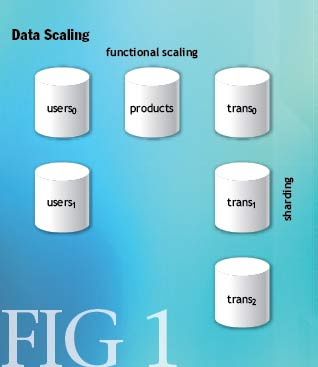
\includegraphics[width=\linewidth]{images/data_scale_base.jpg}
     \caption{Приклад використання шардингу}
     \label{fig:sharding}
\end{figure}

Як показано на діаграмі \ref{fig:sharding}, обидва підходи до горизонтального масштабування можуть застосовуватися відразу. Користувачі, продукти та транзакції можуть бути в окремих базах даних. Крім того, кожна функціональна область може бути розділена між кількома базами даних для транзакційної спроможності. Як показано на схемі, функціональні області можна масштабувати незалежно один від одного.

\paragraph{Функціональне розбиття}

Функціональне розділення важливо для досягнення високих ступенів масштабованості. Будь-яка гарна архітектура бази даних буде розкладати схему на таблиці, згруповані за функціональністю. Користувачі, продукти, транзакції та зв'язок є прикладами функціональних областей. Використання концепцій баз даних, таких як зовнішні ключі, є загальним підходом для підтримки узгодженості в цих функціональних областях.

Спираючись на обмеження бази даних, щоб забезпечити узгодженість між функціональними групами, створюється зв'язок схеми зі стратегією розгортання бази даних. Для обмежень, які повинні застосовуватися, таблиці повинні перебувати на одному сервері бази даних, що виключає горизонтальне масштабування при зростанні швидкості транзакцій. У багатьох випадках найпростішою можливістю масштабування є переміщення функціональних груп даних на дискретні сервери баз даних.

Схеми, які можуть масштабуватися до дуже високих обсягів транзакцій, розміщують функціонально різні дані на різних серверах баз даних. Це вимагає переміщення обмежень даних з бази даних і до програми. Це також вносить ряд проблем, які розглядаються далі в цій статті.

https://queue.acm.org/detail.cfm?id=1394128
\paragraph{Теорема CAP}

Ерік Брюер, професор з Каліфорнійського університету, Берклі і співзасновник і головний науковий співробітник Inktomi, зробив припущення, що веб-служби не можуть забезпечити всі три наступні властивості одночасно (позначені абревіатурою CAP):

Послідовність. Клієнт сприймає, що безліч операцій відбулося відразу.

Доступність. Кожна операція повинна завершитися у передбачуваній відповіді.

Переносимість розділів. Операції будуть завершені, навіть якщо окремі компоненти недоступні.

Зокрема, веб-додаток може підтримувати не більше двох таких властивостей з будь-яким дизайном бази даних. Очевидно, що будь-яка стратегія горизонтального масштабування ґрунтується на розбиранні даних; тому дизайнери змушені вирішувати питання між послідовністю та доступністю.


\subsection{ACID}

ACID (Atomicity, Consistency, Isolation, Durability) — це сукупність властивостей розподіленої бази даних, що гарантують надійну роботу для транзакцій в базі даних: атомарність, узгодженість, ізольованість та довговічність. 

В контексті баз даних, послідовність операцій з базою даних, яка задовольняє властивостям ACID, можна розглядати як одну логічну операцію над даними. Така послідовність операцій називається транзакцією. Наприклад, переказ коштів з одного банківського рахунку на інший, містить численні операції, але є єдиною транзакцією. Отже, розберемо більш детально ці чотири характеристики:

«A» Атомарність (Atomicity) гарантує, що транзакція буде зафіксована тільки повністю, коли виповняться всі її операціїї або не зафіксується, якщо не виповниться якась одна.
NoSQL бази даних, які відповідають іншому принципу BASE (про який ми поговорими пізніше) загалом мають високу продуктивність, бо нехтують цим принципом і не підтримують транзакційну семантику (транзакція потребує багато часу для обробки). 
Багато систем реалізують модулі, які забезпечують такую гарантію: на рівні ключа і рядку (наприклад, Google Big Table) або надають
інтерфейс прикладного програмування для атомарних операцій. За допомогою такого інтерфейсу тільки один потік може модифікувати запис.
Однак більшість систем дотримуються неблокуючих read-modify-write циклів, кожний з яких складається з трьох етапів: прочитати значення, модифікувати його та зберегти зміни.У багатопоточній системі багато чого можуть піти не так, якщо хтось змінить запис між фазами читання і зберігання, наприклад конфлікт записів. Для цієї проблеми винайшли так званий ETag - хеш запису і оновити можна тільки маючи оновлений хеш. У такому разі користувач знає, яку саме інформацію він оновлює.

«C» Узгодженість (Consistency)

Транзакція, яка повністю завершується и фіксує свої результати, зберігає узгодженість бази даних. 
В силу своєї специфіки, NoSQL повинні вибирати високу доступність ( Availability) та здатність до горизонтального масштабування кластера, розподілення інформації по серверам є обов'язковою умовою, що виключає можливість для системи гарантувати, що всі репліки -  копії однієї і тієї ж одиниці даних, мають одну версію і система не може забезпечити повну узгодженість даних та йде на деякі поступки у визначеннях понять узгодженості. Розрізняють декілька видів для узгодженості, які розглядаються окремо у наступній секції.

«I» Изольованість (Isolation)


Під час виконання кржної транзакції параллельні ій транзакції ніяким чином не повинні впливати на результат. Також має значення рівня ізольованності транзакції.

Cassandra, наприклад, починаючи з версії 1.1 гарантує, що якщо ви виконуєте оновлення

\begin{example}

UPDATE Users
SET login='login' AND password='password'
WHERE key='key'

\end{example} ,

то ніякий паралельний потік, який зчитує не зможе побачити часткове оновлення даних (наприклад, зміниться логін, пароль залишиться старим ). Але це працює тількі на рівні текстових значень, які знаходяться у рамках одного  "column family" та мають спільний ключ.

Це може відповідати так званому рівню ізоляції "read uncommitted", де вирішується конфлікти "lost update".
Але Cassandra не надає механізму відкату на рівні кластера. Наприклад, можлива ситуація коли "login" та "password" будуть збережені
на якійсь кількості вузлів, але так кількість буде недостатньою, щоб віддати вірний результат, тобто замало вузлів будуть зберігати
у потрібний час оновлений запис. При цьому користувач буде змушений сам вирішити конфлікт.
Механізм забезпечення ізоляції полягає в тому, що для кожного несталого запису створюється невидима, ізольована для клієнтів версія,
яка згодом заміняє стару за допомогою механізмів Compare and Swap, тобто якщо хтось змінив запис у процесі циклу між читанням і зберіганням запису - система повинна зрозуміти, що на цьому моменті запис змінився та буде повторювати цикл до тих пір, поки наше значення не буде збереженим. Такий алгоритм виглядає більш переважним перед повністю блокуючим записи механізмом. 
Кількість таких циклів може бути великою, тому на такі операції виставляється деякий timeout, по закінченню якого операція буде відхилена.

«D» Надійність (Durability)

Незалежно від проблем на нижніх рівнях (миттєве вимикання системи з різних причин - нестача пам'яті, 
знеструмлення або збій в обладнанні ) зміни, виконані завершеною транзакцією, повинні залишитися в системі збереженими після повернення системи в роботу. Іншими словами, якщо користувач отримав підтвердження від системи, що транзакція була виконана, він може бути впевненим, що його зміни не будуть відхилені системою в ніякому разі.

Забезпечення надійності в рамках одного сервера


Стандартний жорсткий диск (HDD) у середньому витримує 70-150 операцій в секунду, що складає пропускну здатність до 150 Мб/c, 
SSD (solid state drive) — 700 Мб/c, DDR (double data rate) у модулы оперативної пам'яті — 6000 — 17000 Мб/c. 
Тому забезпечення надійності в рамках одного сервісу при забезпеченні високої продуктивності є зменшення кількості записів з 
доступом до випадкового місця в пам'яті та збільшення послідовного запису, де навідник (pointer) вже відомий.
В ідеалі, система повинна мінімізувати число записів між системними виклаками fsync (синхронізація даних в пам'яті і на диску).
Для цього застосовують декалька технік:

\begin{itemize}

\item Контроль частоти викликів fsync

Redis пропонує кілька шляхів для налаштування такої частоти. Можна сконфігурувати, щоб fsync викликався після кожної зміни запису,
що є найповільнішим і найбезпечнішим шляхом. Щоб покращити продуктивність, можна вибирати інтервал між викликами кожні N секунд,
у гіршому випадку ви втрачаєте дані за N останніх секунд, тому таке число можна вибрати самому залежно від певних потреб.

\item Збільшення послідовного запису через журналювання (logging)

Для ефективного пошуку даних NoSQL системи часто використовують додаткові структури, наприклад, B-дерева для побудови індексів, робота 
з індексами приводить до баготочисленних випадкових доступів до диску. Для зменшення цього деякі системи додають операції
оновлення у файл послідовного запису, що зветься $redo log$. Поки структури пишуться на диск, пишеться лог і після падіння
бракуючі записи можна відновити за допомогою лога.

\item Збільшення пропускної здатності групуванням записів

Cassandra групує кілька одночасних змін, які можуть бути об'єднані у один fsync. Такий підхід, що зветься $group commit$,
збільшує час відклику для одного користувача, оскільки він вимушений чекати на інші транзакції для того, щоб зафіксувати власну.
Цей метод перважний через збільшення загальної пропускної здатності в підсумку, оскільки кілька випадкових записів можуть бути об'єднані.

\item Обеспечение надёжности в рамках кластера серверов

Через можливість непередбачуваних виходів з ладу дисків та серверів є необхідним розподіляти інформацію на кілька машин.
Так, Redis представляє собою класичну master-slave архітектуру для репликації даних. Всі операції, зв'язані з мастером,
користуються репліками у вигляді логу.

MongoDB являє собою структуру, в якій задана кількість серверів зберігає кожний документ, причому є
можливість задати кількість серверів $W < N$, де $N$ - загальна кількість серверів у розподіленій мережі, а $W$ - достатня кількість,
яка є мінімально необхідною для запису та повернення керування користувачу.
HBase досягає мультисерверної надійності за рахунок розподіленої файлової системи HDFS.

\end{itemize}
https://habr.com/en/post/228327/

Компанії, продуктом якиз є бази даних, давно визнали необхідність розбиття баз даних і впровадили техніку, відому як 2PC (two-phase commit), для забезпечення гарантій ACID для декількох екземплярів бази даних. Протокол розбитий на дві фази:
\begin{itemize}
\item По-перше, координатор транзакцій просить кожну задіяну базу даних попередньо вказати, чи є можливим фіксація перед виконанням операції. 
Якщо всі бази даних погоджуються, що фіксація може продовжуватися, починається фаза 2.
\item Координатор транзакцій запитує кожну базу даних для фіксації даних.
\end{itemize}

Якщо будь-яка база даних накладає вето на фіксацію, то всі бази даних просять відкатити (rollback) свої частини транзакції. Однак є недолік в тому, що ми отримуємо узгодженість між так званими "partitions" баз даних. Якщо Brewer правий, то це повинно впливати на доступність (availability), але яким чином?

Доступність будь-якої системи - доступность кожного з її компонентів, необхідних для проведення операцій над системою. 
Остання частина цього твердження є найбільш важливою. Компоненти, які можуть використовуватися системою, але не потрібні, не зменшують доступність системи. Транзакція, що включає дві бази даних в 2PC комміті, доступна, якщо є необхідні дані в кожній базі даних. 
Наприклад, якщо припустити, що кожна база даних має 99,9 \% доступності, то доступність транзакції дорівнює 99,8 \%, також в базі даних наявний додатковий час простою 43 хвилини на місяць.

\subsection{BASE як протиставлення ACID} 

Якщо ACID забезпечує вибір узгодженості для розділених баз даних, то як замість цього досягти доступності? 
Однією з відповідей є BASE (Basically Available, Soft state, Eventually consistent).

Принцип BASE є діаметрально протилежним ACID. Там, де ACID є песимістичним і зумовлює узгодженість в кінці кожної операції, BASE є оптимістичним і приймає, що узгодженість бази даних буде перебувати у стані потоку і зрештою зійдеться. 
Хоча це звучить неможливо, але насправді воно досить кероване і призводить до рівнів масштабованості, які неможливо отримати за допомогою ACID.

Доступність BASE досягається шляхом підтримки часткових відмов без повної відмови системи. Ось простий приклад: якщо користувачі розділені на п'ять серверів баз даних, дизайн BASE заохочує створення операцій таким чином, що збій бази даних користувачів впливає лише на 20 \% користувачів цього конкретного хоста. Це призводить до більш високої доступності системи.
Отже, тепер, коли ви розклали ваші дані на функціональні групи і розділили найважчі групи на декілька баз даних, як ви включаєте BASE у вашу програму? BASE вимагає більш глибокого аналізу операцій в рамках логічної транзакції, ніж зазвичай застосовується до ACID. Що потрібно шукати? Наступні розділи надають певний напрямок.

\paragraph{Шаблони узгодженості}

Після гіпотези Брюєра, якщо BASE допускає наявність в розділеній базі даних, то необхідно ідентифікувати можливості для послаблення узгодженості. Це часто буває важко, оскільки тенденція потреб як зацікавлених сторін бізнесу, так і розробників полягає в тому, що послідовність має першорядне значення для успіху програми. Тимчасова невідповідність не може бути прихована від кінцевого користувача, тому власники машинобудування та продуктів повинні бути залучені до вибору можливостей для ослаблення узгодженості таким чином, щоб це задовільнило обидві сторони.

\begin{figure}
\centering
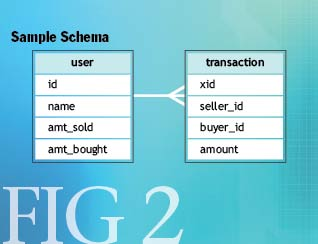
\includegraphics[width=\linewidth]{images/sample_schema.jpg}
     \label{fig:sample_schema}
\end{figure}

Малюнок \ref{fig:sample_schema} - це проста схема, яка ілюструє принцип узгодженості для BASE. Таблиця клієнта банку 
містить інформацію про користувача, включаючи загальну списану та придбану суму. 
Це загальні підсумки. У таблиці транзакцій зберігається кожна транзакція, що стосується продавця і покупця і суми операції. 
Це великі спрощення реальних таблиць, але містять необхідні елементи для ілюстрації декількох аспектів узгодженості.

Загалом, узгодженість між функціональними групами легше послабити, ніж всередині функціональних груп. Приклад схеми має дві функціональні групи: користувачі та транзакції. Щоразу, коли товар продається, в таблицю транзакцій додають рядок, а лічильники для покупця і продавця оновлюються. Використовуючи підхід ACID, SQL буде таким, як показано на малюнку \ref{fig:sql_query}.

\begin{figure}
\centering
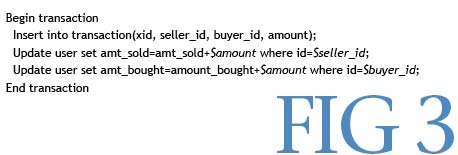
\includegraphics[width=\linewidth]{images/sql_query.jpg}
     \label{fig:sql_query}
\end{figure}

Загальна кількість "куплених" і "проданих" стовпців у таблиці користувачів може розглядатися як кеш таблиці транзакцій. 
Він присутній для ефективності системи. Враховуючи це, обмеження на узгодженість може бути зменшено. Очікування покупця і продавця можуть бути встановлені таким чином, щоб їхні поточні залишки не відображали результат операції одразу. 
Це не рідкість, і насправді люди стикаються з такою затримкою між операцією та поточним балансом (наприклад, зняття банкоматів та дзвінки з мобільного телефону).

Як змінюються оператори SQL, щоб послабити узгодженість, залежить від того, як визначаються поточний залишок. Якщо вони просто оцінюються і не мають великого значення, то деякі транзакції можуть бути пропущені, зміни досить прості, як показано на малюнку \ref{fig:transaction}.

\begin{figure}
\centering
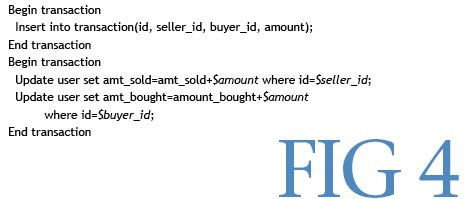
\includegraphics[width=\linewidth]{images/transaction.jpg}
     \label{fig:transaction}
\end{figure}

Тепер уявимо, що ми роз'єднали оновлення для користувачів і таблиці транзакцій. Узгодженість між таблицями не гарантується. Фактично, відмова між першою і другою транзакцією призведе до того, що таблиця користувача буде постійно несумісною, але якщо контракт передбачає, що поточні підсумки є неважливими, це може бути адекватним.

Що робити, якщо оцінки не є прийнятними? Як ви все ще можете роз'єднати оновлення користувачів і транзакцій? Введення постійної черги повідомлень вирішує проблему. Існує декілька варіантів реалізації постійних повідомлень. ирішальним фактором у реалізації черги є забезпечення того, щоб збереження резервної копії знаходилося на тому ж ресурсі, що й база даних. Це необхідно для того, щоб дозволити черзі здійснювати транзакції без залучення 2PC. Тепер операції SQL виглядають дещо іншим, як показано на малюнку \ref{fig:transaction_2}.

Цей приклад дає певні свободи синтаксисом і спрощує логіку для ілюстрації цієї концепції. Очікуючи постійне повідомлення в тій самій транзакції, що й вставка, інформація, необхідна для оновлення поточних балансів користувача, була захоплена. Транзакція міститься в одному екземплярі бази даних і тому не вплине на доступність системи.

\begin{figure}
\centering
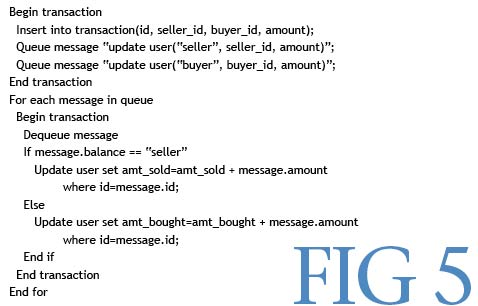
\includegraphics[width=\linewidth]{images/transaction_2.jpg}
     \label{fig:transaction_2}
\end{figure}

Окремий компонент обробки повідомлень видалятиме кожне повідомлення з черги і застосовуватиме інформацію до таблиці користувачів. Наведений приклад вирішує всі питання, але є проблема. Повідомлення зберігається на сервері, де виконується транзакція, щоб уникнути 2PC під час чергування. Якщо повідомлення видаляється в транзакції з використанням хоста користувача, ми все ще маємо ситуацію двухфазного комміту (2PC).

Одне з рішень для 2PC в компоненті обробки повідомлень - нічого не робити. Виносячи оновлення запису в окремий компонент back-end, ви зберігаєте доступність компонента, що стоїть перед клієнтом. Більш низька доступність процесора повідомлень може бути прийнятною для бізнес-вимог.

Припустимо, однак, що техніка двухфазного комміту 2PC просто не прийнятна у вашій системі. Як вирішити цю проблему? 
По-перше, дамо визначення такому поняттю, як ідемпотентність. Операція вважається ідемпотентною, якщо її можна застосувати один раз або кілька разів з однаковим результатом. Ідемпотентні операції корисні тим, що вони допускають часткові відмови, і застосування їх неодноразово не змінює кінцевого стану системи.

Однак вибраний приклад на Малюнку \ref{fig:transaction_2} є проблематичним при застосуванні ідемпотентності. 
Операції по оновленню рідко є ідемпотентними. Наданий приклад інкрементить значення у колонці балансу. 
Неодноразове застосування цієї операції призведе до неправильного балансу. 
Проте навіть найпростіші операції оновлення, які просто встановлюють одне значення, не є ідемпотентними щодо порядку операцій.
Якщо система не може гарантувати, що оновлення будуть застосовані в тому порядку, в якому вони отримані, остаточний стан системи буде неправильним.

У разі оновлення балансу потрібен спосіб відстежувати, які оновлення були успішно застосовані, а які ще залишаються невиконаними. 
Одним з методів є використання таблиці, яка записує ідентифікатори транзакцій, які були застосовані.

\begin{figure}
\centering
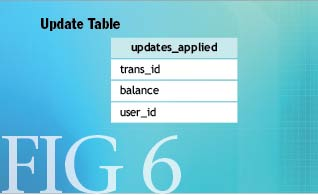
\includegraphics[width=\linewidth]{images/fig6.jpg}
     \label{fig:fig_6}
\end{figure}

Таблиця, показана на \ref{fig:fig_6}, відстежує ідентифікатор транзакції, в якої був оновлений баланс, і ідентифікатор користувача, для якого був оновлений баланс. Тепер зразок псевдокоду для работу з такою таблицею представлений на малюнку \ref{fig:fig_7} .

\begin{figure}
\centering
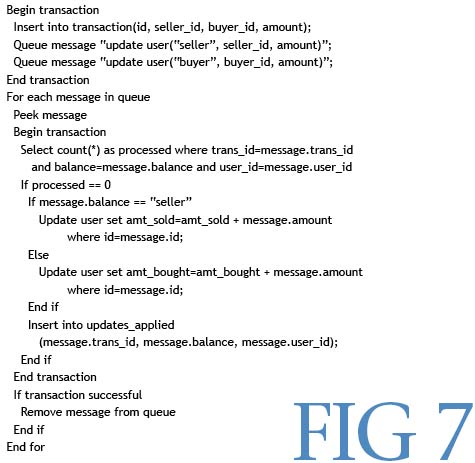
\includegraphics[width=\linewidth]{images/fig7.jpg}
     \label{fig:fig_7}
\end{figure}

Цей приклад залежить від можливості взяти повідомлення в черзі і видалити його після успішної обробки. 
Це можна зробити за допомогою двох незалежних транзакцій, якщо необхідно: один на черзі повідомлень і один на базі даних користувача. 
Операції на черзі не виконуються, доки операції з базами даних не успішно завершені.
Алгоритм тепер підтримує часткові відмови і все ще забезпечує транзакційні гарантії, не вдаючись до двухфазного коміту 2PC.

Існує більш проста техніка для гарантії ідемпотентних оновлень, але при цьому має бути тільки одна єдина вимога, яка полягає в упорядкуванні. 
Таке рішення ілюструє Малюнок \ref{fig:fig_8}). 
Припустимо, ви також хочете відстежувати останню дату продажу та покупки для користувача. 
Можна покластися на подібну схему оновлення дати з повідомленням, але треба враховувати декілька деталей.


\begin{figure}
\centering
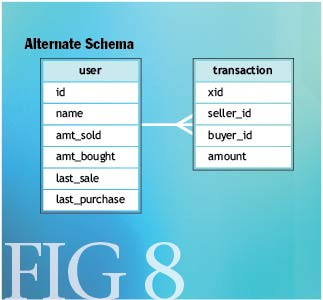
\includegraphics[width=\linewidth]{images/fig8.jpg}
     \label{fig:fig_8}
\end{figure}

\begin{figure}
\centering
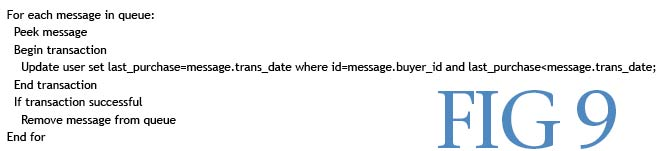
\includegraphics[width=\linewidth]{images/fig9.jpg}
     \label{fig:fig_9}
\end{figure}

Припустимо, що дві покупки відбуваються протягом короткого часового вікна, і наша система повідомлень не забезпечує впорядкованих операцій. Тепер ви маєте ситуацію, коли в залежності від того, в якому порядку обробляються повідомлення, ви матимете неправильне значення колонки $last_purchase$ (остання оплата). 
На щастя, цей вид оновлення може бути оброблений з незначною модифікацією SQL, як показано на малюнку \ref{fig:fig_9}.

Отже, якщо не дозволяти значенню в колонці $last_purchase$ йти назад у часі, порядок операцій оновлення буде незалежним.
Ви також можете використовувати цей підхід для захисту будь-яких оновлень від оновлень поза замовленням. Як альтернативу використання часу, 
можна також спробувати постійно робити операцію інкременту над ідентифікатором транзакції.

\paragraph{Впорядкування черги повідомлень}

Актуально зауважити додаткову інформацію щодо впорядкованої доставки повідомлень. 
Системи черг повідомлень надають можливість гарантувати, що повідомлення доставляються в тому порядку, в якому вони отримані. 
Але це дуже важко підтримувати і часто є непотрібним, і, по суті, часом дає помилкове почуття безпеки, якщо є помилка у налаштуванні такої системи.

Наведені тут приклади ілюструють, як впорядкування повідомлень може бути послаблене і, як і раніше, забезпечувати послідовний вигляд бази даних. 
Накладні витрати, необхідні для розслаблення впорядкування, номінальні, і в більшості випадків значно менше, ніж примусове впорядкування в системі повідомлень.

Крім того, веб-додаток є семантично системою, керованою подіями, незалежно від стилю взаємодії. Запити клієнта надходять до системи у довільному порядку. 
Час обробки, необхідний для кожного запиту, змінюється. Планування запитів по всіх компонентах систем є недетермінованим, 
що призводить до недетермінованого чергування повідомлень. Вимоги до збереження наказу дають помилкове почуття безпеки. Проста реальність полягає в тому, що недетерміновані входи призведуть до недетермінованих результатів.

\paragraph{Soft State / Eventually Consistent}

До недавніх часів акцент робився на узгодженості і узгодженість переважала доступність. З іншого боку, треба бати до уваги вплив принципу "soft state"
та "eventual consistency" мають на розробку додатків.

Як інженери ми схильні розглядати наші системи як замкнутий ланцюжок. 
Ми думаємо про передбачуваність їхньої поведінки з точки зору передбачуваних входів, що виробляють передбачувані результати. Це необхідність створення правильних програмних систем. Хороша новина у багатьох випадках полягає в тому, що використання BASE не змінює передбачуваності системи як замкнутого циклу, але вимагає перегляду загальної поведінки.

Простий приклад може допомогти проілюструвати це. Розглянемо систему, в якій користувачі можуть передавати активи іншим користувачам. Тип активу не має значення - це можуть бути гроші або об'єкти в грі. 
У цьому прикладі ми припустимо, що ми відокремили дві операції: прийом активу від одного користувача та передача активу іншому з чергою повідомлень.

Відразу ця система вже здається недетермінованою і проблематичною. Існує певний період часу, коли актив залишив одного користувача та ще не прибув до іншого. Розмір цього часового вікна може бути визначений за допомогою системи обміну повідомленнями. 
Незважаючи на це, існує відставання між стартовим і кінцевим станами, де жоден користувач не має активу.

Однак, якщо розглядати це з точки зору користувача, ця затримка може бути нерелевантною для нього або навіть відомою. 
Ні одержувач, ні відправник не можуть знати, коли приїхав актив. 
Якщо відставання між відправленням та отриманням становить кілька секунд, воно буде непомітним або, звичайно, допустимим для користувачів, які безпосередньо повідомляють про передачу активів. У цій ситуації поведінка системи вважається послідовною і прийнятною для користувачів, навіть якщо ми покладаємося принцип
"soft state / eventually consistent" у реалізації.

\paragraph{Архітектура, керована подіями}

Але що робити, якщо ви повинні чітко знати, коли поведінка системи стала послідовною? 
Ви можете мати алгоритми для визначення стану системи, але тільки тоді, коли вона досягла стабільного стану, відповідного вхідному запиту. 
Підхід полягає в тому, щоб покладатися на події, які генеруються, як тільки стан стає послідовним.

Продовжуючи попередній приклад: що, якщо вам потрібно повідомити користувача, що актив прибув? Створення події в транзакції, яка здійснює передачу активу в користувачу-одержувачу, забезпечує механізм для здійснення подальшої обробки після досягнення відомого стану. EDA (заснована на подіях архітектура) може забезпечити різке поліпшення масштабованості та архітектурної розв'язки. Подальша дискусія щодо застосування EDA виходить за рамки цієї статті.

\paragraph{Висновок}

Масштабування систем до значних частот транзакцій вимагають нового способу управління ресурсами. 
Традиційні транзакційні моделі є проблематичними, коли навантаження необхідно розподілити між багатьма компонентами. Від'єднання операцій і виконання їх у свою чергу забезпечує покращення доступності та масштабу за рахунок узгодженості. BASE надає моделі рішення до цього розподілення.


 \section{Розподілені бази даних та їх типи узгодженості}

Розподілена база даних (або розподілене сховище даних) — це сукупність логічно взаємопов'язаних баз даних, розподілених у комп'ютерній мережі. Логічний зв'язок баз даних в розподіленій базі даних забезпечує система управління розподіленою базою даних, яка дозволяє управляти розподіленою базою даних таким чином, щоб створювати у користувачів ілюзію цілісної бази даних. 


Для будь-якої розподіленої бази даних існують такі властивості, встановлених К.Дейтом (див. \cite{bib:database_principles} :
\begin{itemize}
 \item Локальна автономія. Вона означає, що управління даними в кожному вузлі виконується локально і незалежно від інших вузлів системи
 \item Незалежність вузлів. Вважається, що в ідеальній системі всі вузли рівноправні і незалежні, а бази даних є рівноправними постачальниками інформації в загальний інформаційний простір.
 - Прозорість розміщення даних. Користувач не мусить знати де розміщені дані. Під час роботи створюється враження, що дані знаходяться саме на його комп’ютері.
 - Прозора фрагментація. Ця властивість трактується, як можливість створення фізично розподілених даних, які логічно утворюють єдине ціле. Допускається горизонтальна та вертикальна фрагментація.
 - Прозорість тиражування. Забезпечує тиражування (перенос змін) об’єктів первинної бази даних в усі вузли її розміщення внутрішньосистемними засобами.
 - Обробка розподілених запитів. Означає виконання операцій, сформованих, в рамках звичайного запиту на мові SQL.
 - Обробка розподілених транзакцій. Забезпечує виконання операцій з одночасним забезпеченням цілісності і узгодженості даних, шляхом використання двофазового протоколу фіксації транзакцій.
 - Незалежність від обладнання. Для оснащення вузла можуть використовуватися комп’ютери різних марок і виробників.
 - Незалежність від операційних систем. Передбачає допустимість взаємодії різноманітних операційних систем у різних вузлах розміщення розподіленої бази даних.
 - Прозорість мережі. Забезпечує будь-які протоколи в локальній обчислювальній мережі, яка обслуговує розподілену базу даних.
 - Незалежність від типу баз даних. Допускає співіснування різних систем керування базами даних.
 - Неперервність операцій. Дані доступні завжди, а операції над ними проводяться неперервно.

\end{itemize} 
http://citforum.ru/database/kbd96/45.shtml
Також для розподіленої бази даних існують три найважливіші парадигми, за допомогою яких підтримується ефективна робота для користувача:
\begin{itemize}
\item[Цілісність] Це складна проблема в розподіленій системі даних. Її рішення - синхронна і узгоджена зміна даних у кількох локальних базах даних, які скаладають розподілене сховище, і воно досягається застосуванням протокола фіксації транзакцій. Але це може застосовуватися у випадку, якщо база даних однородна. Якщо розподілена БД неоднородна, для цього використовують механізми розподілених транзакцій. Проте, це можливо при підтримці ХА-інтерфейсу учасниками обробки розподіленої транзакції, які функціонують на вузлах системи,   Это, однако, возможно, если участники обработки распределенной транзакции - СУБД, функционирующие на узлах системы. ХА-інтерфейс визначений в специфікації DTP консорціума X/Open. Нині XA-інтерфейс підтримується CA-OpenIngres, Informix, Microsoft SQL Server, Oracle, Sybase.
Якщо в розподіленому сховищі передбачено тиражування даних, це одразу пред'являє жорсткі  вимоги до підтримки цілісності на вузлах, куди направляються потоки тиражованих даних. То ж конфлікти щодо змін, які необхідно відслідковувати, неминучі. 
\item[Узгодженість] Як і у всіх інших розподілених систем, одним з основних компонентів цілісності даних (цілісності системи) є узгодженість - гарантія того, що усі вузли бачать однакові дані на будь-який момент часу.
Підтримка узгодженості в базах даних є ключовою при стабільній роботі розподіленого сховища даних. 
За узгодженістю слідують доступність даних (в будь-який момент кліент може отримати дані зі сховища або відповідь про те, що їх нема, за розумний обсяг часу) і стійкість до розділення системи (не зважаючи на розділення на ізольовані секції або втрати зв'язку з частиною вузлів, система не втрачає стабільність і здатність коректно відповідати на запити).

\end{itemize}

{\bfseries{red} Реплікація з книжки Таненбаума}
Є відома теорема CAP, яка наголошує, що з трьох властивостей (узгодженість (consistency), доступність (availability), стійкість до розділення (partition tolerance)) неможливо забезпечити більше двох в одній і тий самій конфігурації системи: наприклад, якщо забезпечити узгодженість, втратиться одна з двох інших властивостей. 

Крім того, в цій роботі важливо зазначити, що розділяють наступні моделі узгодженості:

\begin{itemize}
\item Сувора узгодженість (несуперечливість) (Strong Consistency) - на будь-який запит на читання елемента даних $x$ сховище дає значення, які відповідає наойновішої версії. Це найжорсткіша, але модель несуперечливості для підтримки абсолютної узгодженості, і її забезпечення до втрачання вкличини доступності для даної конфігурації сховища даних.

\item Послідовна несуперечливість (sequential consistency) - результат будь-якої дії такий же, якщо б операції читання та запису всіх процесів у сховище даних виконувались би в деякому послідовному порядку і притому операції кожного окремого процесу виконувались би у порядку, визначеного його програмою. Тобто будь-яке правильне чередування операцій читання и запису є допустимим , але всі процеси бачать одне и те ж чередування операцій.

\item Причинна несуперечливість (causal consistency) - операції на запис, які потенціально зв'язані причинно-наслідковим зв'язком, повинні  обслуговуватися всіма процесами в одному і тому ж порядку, а паралельні записи можуть параллельно обслуговуватися на разних вузлах в різному порядку.

\item Несуперечливість FIFO. Операції запису, які здійснюються поодиноким процесом, розглядаються іншими процесами в тому порядку, в якому вони здійснюються, але операції запису з різних процесів, можуть спостерігатися різними процесами у різному порядку.

\item Потенціальна несуперечливість - при відсутності змін всі репліки поступово стають несуперечливими. Такі моделі використовуються, коли клієнт запрошує завжди одну й ту ж репліку та записи в таке сховище виконуються нечасто.

\end{itemize}

Забезпечення суворої узгодженості - занадто дорога модель для будь-якої розподіленої бази даних, хоча деякі бази це забезпечують, для яких застосування такої моделі - сувора технічна вимога, що випливає з бізнес-логіки продукту, де така база використовується.
Але такі конфігурації розподілених БД втрачають значення іншої характеристики - доступності даних, бо для великих БД потрібно багато часу, щоб досягнути суворої несуперечливості і клієнт змушений чекати, щоб мати гарантію на отримання несуперечливих актуальних даних.

Ми намагаємося знайти компроміс, щоб максимально близько реалізувати таку модель без втрачання доступності і стійкості до розділення розподіленої бази (див. модель реалізації  у наступних частинах).

\section{Протоколи поширення реплік між вузлами розподіленої бази даних}
GOSSIP, ...
\section{Балансування навантаження}

Балансувальник навантаження - це метод, який дозволяє розподіляти задачі між мережевими пристроями з метою оптимізації використання ресурсів, збереження часу відопвіді на запити, горизонтального масштабування кластеру та забезпечення відмовостійкості розп%оділеної системи. Прикладами пристроїв, до яких може бути застосований цей метод, є серверні кластери, проксі-сервери, межмережеві екрани, комутатори, сервери інспектування вмісту, сервери DNS, мережеві адаптери. Балансувальник запиту може бути застосований у різних цілях, також деякі реалізації балансування - проекти з відкритими джерелами, які дозволяють дописати необхідний функціонал для перенаправлення запитів за необхідним алгоритмом, допрацювати існуючі алгоритми та інше (HAProxy, Nginx, Seesaw, Zevent, Neutrino, Traefik, тощо https://geekflare.com/open-source-load-balancer/).
\begin{figure}
\centering
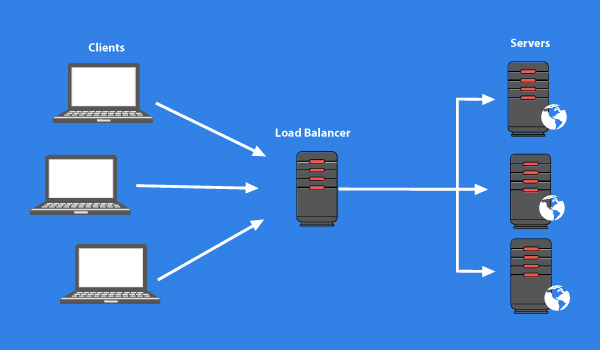
\includegraphics[width=\linewidth]{images/load-balancing-general.jpg}
     \caption{Загальна архітектура балансування навантаження.}
     \label{fig:lb_general}
\end{figure}

Малюнок \ref{fig:lb_general} демонструє загальний механізм роботи  балансувальника навантаження: запит приходить спочатку на проміжний вузел (або кластер) і далі  перенаправляється на один з вузлів в системі, який спроможний відповісти на запит клієнта. Періодично балансувальник робе так званий "healthcheck", щоб вчасно мати знання про те, які вузли зможуть відповісти на запит.
Балансування може здійснятися за різними додатковими характеристиками: запит відправиться на найбільш незайнятий вузел, на вузел, який за показниками процесора на даний момент часу має не завантажений процесор, тощо. 

Алгоритми балансування навантаження загалом можна класифікувати наступним чином (Малюнок \ref{fig:lb_classification}):

\begin{figure}
\centering
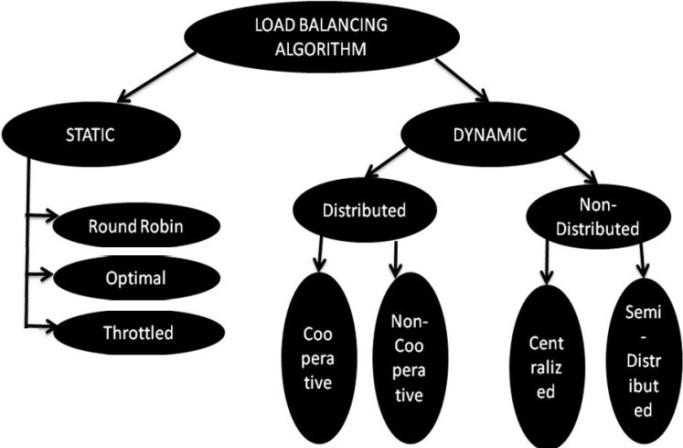
\includegraphics[width=\linewidth]{images/Classification-of-load-balancing-algorithms-in-cloud.png}
     \caption{Класифікація алгоритмів балансування навантаження.}
     \label{fig:lb_classification}
\end{figure}

Ці алгоритми спершу розділяють на статичні і динамічні:

\begin{enumerate}
\item Статичне балансування. В цьому підході балансування навантаження реалізується через забезпечення важливої інформації про систему. Визначається продуктивність вузла на початку виконання операцій. Вузли виконують обчислювання та надають результати на інші вузли. Потім задачі розподіляються на початку, не зважаючи на те, як вже навантажені вузли. [13]
Статичні методи балансування повтодяться таким чином, що якщо вже якийсь вузел виділений для певного процесу, процес не може бути перерозподіленим на інший вузол.
Ций метод потребує менше взаємодії, отже зменшує час виконання операцій. [16]
Однак основна перешкода цього підходу - механізм не зважає на поточний стан системи, коли розподіляє задачі на вузли.
Це має значний вплив на продуктивність всієї розподіленої системи через велику амплітуду коливання навантаження в системі. [18]. 
Є чотири типи статичних алгоритмів балансування навантаження: циклічного планування (Round Robin), Центральний менеджер (Central Manager), 
Алгоритм Порогу (Threshold Algorithm) та рандомізований алгоритм (randomized):

\begin{itemize}

\item a)  Алгоритм циклічного планування (Round Robin)  [12]. В цьому алгоритмі навантаження розподіляється рівномірно на всі вузли мережі, де рівне навантаження призначається у кільцевому порядку без будь-якого пріорітету та повертається у кінці на перший вузел, якщо останній вузел був доступним. 
Кожний вузел  виконує свою роботу, яка була для нього виділена, незалежно від розташування інших вузлів. Алгоритм циклічного планування простий у роботі, легко реалізовується, також ситуації "голодування" (коли вузел простоює, не виконує жодних процесів, що приводить до неефективного використання).  
Цей алгоритм не потребує комунікації між процесами та дає кращу продуктивність для додатків спеціального призначення. 
Однак алгоритм не може дати очікуваний результат в загальному випадку і коли процеси потребують різної кількості часу для виконання. 

\item b) Алгоритм "Центральний менеджер" (Central Manager Algorithm) [16]: В цьому алгоритмі центральний вузол вибирає інший, який називають "slave" 
для того, щоб "slave" взяв навантаження на себе. Навантаження призначаэться тому вузлу типу "slave", який має у цей момент часу найменше навантаження.
Центральний вузол підтримує індекс навантаження всіх вузлів типу "slave", які приєднані к центральному. 
Кожний раз, як міняється навантаження, всі вузли отримують повідомлення про це від центрального вузла. Цей алгоритм потребує високий рівень комунікації між вузлами, який іноді може привести до стану "вузького місця" (bottleneck), коли навантаження на вузел занадто велике, та вузел не може впоратися і відповідати всім вузлам.   Цей алгоритм має кращу продуктивність, коли динамічні активності створюються різними вузлами. 
\item c) Алгоритм Порогу (Threshold Algorithm) [13]: Відповідно до цього алгоритму навантаження призначається одразу на створенні вузла. Вузли вибираються локально без відправки повідомлень на інші вузли. Кожний вузел зберігає приватну копію навантаження системи. Навантаження характеризується трьома рівнями: недостатнє (under loaded), середнє навантаження (medium) та перенавантаження (overloaded). Два параметри $t_{under}$ та $t_{upper}$ використовуються для описання цих рівней:


Under loaded - load  $ < t_{under} $


Medium - $t_{under} \leq load \leq t_{upper}$


Overloaded - load $ > t_{upper}$


Від самого початку передбачається, що вузли мають недостатнє завантаження. Коли стан навантаження вузлу перевищує перевищує межу на певному вузлі, цей вузол надсилає повідомлення щодо нового стану навантаження всім віддаленим вузлам, регулярно оновлюючи їх про поточне навантаження. Якщо стан локального вузлу не є перезавантеженим, то навантаження виділяється локально. В іншому випадку вибирається віддалений недозавантажений вузол, і якщо такого вузла немає, робота теж розподіляється локально. Цей алгоритм має низький рівень взаємодії між процесами та великою кількістю локальних розподілів процесів. Пізніше зменшується накладні витрати на віддалений розподіл процесів та накладні витрати на доступ до віддаленої пам'яті, що призводить до поліпшення продуктивності.

\item d) Рандомізований алгоритм [15]: в цьому алгоритмі вузол вибирається випадково, без будь-якої інформації про поточне або попереднє навантаження на вузол. Оскільки алгоритм має статичний характер, він найкраще підходить, коли система має однаковий рівень навантаження на кожен вузол. Дає найкращу продуктивність для спеціальних додатків, які відповідають такій вимозі достатньо рівномірного завантаження. Кожен вузол зберігає власну кількість завантажень, тому не вимагається взаємодії між процесами. Але іноді це може спричинити перевантаження одного вузла у той час, коли інший вузол недостатньо навантажений.
\end{itemize} 


\item Динамічне балансування. Такі алгоритми мають систему моніторінгу за змінами в системі та перерозподіляють процеси відповідно до актуальних даних, які може надати моніторінг. Зазвичай цей алгоритм складається з трьох стратегій: стратегія передачі, стратегія розташування та інформаційна стратегія.
Стратегія передачі вирішує які задачі можуть передати дані на інші вузли для  обробки. Стратегія розташування призначає віддалений вузел виконати завдання.
Інформаційна стратегія - інформаційний центр для алгоритма балансування навантаження [24]. Ця стратегія є відповідальною за забезпечення ресурсів для стратегій розташування та передачі для кожного вузла. Динамічні алгоритми можуть контролювати систему у трьох формах: централізованій, розподіленійта полурозподіленій.
В централізованій розподілення, один центральний вузел в мережі призначається відповідальним за весь розподіл навантаження в мережі. В розподіленій відповідальність розділена між всіма вузлами равномірно [24]. В полурозподіленій мережа сегментується на кластери, де кожний кластер в сегменті централізований.
Балансування навантаження досягається за допомогою кооперації центральних вузлів всіх кластерів [24]. Є три типа динамічних алгоритмів: центральна черга (central queue), локальна черга (local queue) та найменше з'єднання (least connection).

\begin{itemize}

\item a) Алгоритм центральної черги (Central Queue Algorithm) [13]: Цей алгоритм зберігає нову активність (тобто, нові з'єднання) та невиконані запити в циклічній черзі FIFO. Кожна нова активність стає в чергу. Тоді, коли отримують запит на активність, перша активність видаляється з черги. Якщо в черзі немає бажаної активності, запит буферизується, доки не буде доступна нова активність. Це централізований ініціативний алгоритм і потребує високої комунікації між вузлами.

\item b)  Алгоритм локальної черги (Local  Queue  Algorithm ) [16]: цей алгоритм підтримує міграцію між процесами. Ця ідея полягає в статичному виділенні всього нового процесу з міграцією процесів, ініційованої хостом, коли його завантаження потрапляє до вузлу, де заздалегідь визначено мінімальну кількість готових процесів. Коли хост недостатньо завантажений, він запитує про діяльність віддалених вузлів. Віддалені хости потім займаються пошуком свого локального списку для готових процесів, а деякі процеси передаються хосту запитувача та отримують підтвердження від хоста. Такі розподілені кооперативні алгоритми вимагають взаємодії між процесами, але менше, ніж в алгоритмі центральної черги.

\item c)  Алгоритм найменшого з'єднання (Least  Connection  Algorithm ) [24]: цей алгоритм вирішує , як розподіляти навантаження на основі з'єднань, 
присутніх на вузлі. Балансувальник навантаження підтримує журнал повідомлень про з'єднання на кожному вузлі. Число повідомлень збільшується, коли новий
зв'язок встановлюється і зупиняється, коли підключення завершується або закінчується час. Спочатку виділяються вузли з найменшою кількістю з'єднань.

\end{itemize}
\end{enumerate}

\chapter{Метріки властивостей розподіленого сховища даних}

На початку роботи над темою дисертації на основі математичної моделі, яка представлена нижче, були сформовані метріки для основних властивостей розподіленого сховища даних: 
узгодженості, доступності даних, стійкості до розділення (дивиться повну версію 
%https://www.researchgate.net/profile/Vyacheslav_Kharchenko/publication/281447001_Proc_11th_Int_Conf_on_ICT_in_Education_Research_and_Industrial_Applications_Integration_Harmonization_and_Knowledge_Transfer/links/56c1a82f08aee5caccf81ebe.pdf#page=537 
). 

Отже, нехай модель розподіленої бази даних - кортеж $(N, L, \partial,D, r)$, де \\

\begin{tabular*}{\textwidth}{cp{0.5cm}p{0.8\textwidth}}
$N$&& кінцева множина, елементи якої відповідають за вузли (сервери) розподіленого сховища даних; \\
$L$&& кінцева множина, елементи якої відповідають за зв'язки між вузлами розподіленого сховища даних; \\
$\partial:L\rightarrow 2^N$&& відображення, яке ставить у відповідність кожному зв'язку два з ним суміжних вузла;\\
$D$&& кінцева множина, елементи якої відповідають за збережені одиниці даних (dataunits);\\
$r:D\rightarrow 2^N$&& відображення, що ставить у відповідність кожної одиниці даних $d$ підмножину вузлів, які зберігають репліку одиниці даних $d$.
\end{tabular*}


Тепер після опису моделі можемо перейти до метрік. Спершу представимо метріку узгодженості.
Нагадаємо, що узгодженість - це властивість сховища, коли для кожної одиниця даних її репліки, що зберігаються на вузлах, 
мають одне і те ж значення. Ми розглядатимемо випадок, коли всі одиниці даних у розподіленому сховищі узгоджені. Тому метріка узгодженості ми пропонуємо визначати наступним чином:

\begin{definition}[Метріка узгодженості]
Нехай $\sigma_t\in\{0,1\}$ - випадкове значення від 0 до 1, яке  представляє одну з подій у момент часу $t\geq 0$.  Тоді:\\
\begin{tabular*}{\textwidth}{p{0.5cm}cp{0.5cm}p{0.8\textwidth}}.

&$\sigma_t=0$ && змінна, що відповідає за подію ``є одиниця даних, що не є узгодженою 
у момент часу $t$'' та\\
&$\sigma_t=1$ && змінна що відповідає за подію ``всі одиниці даних узгоджені у момент часу $t$''.
\end{tabular*}
Then the consistency metric $C(t)$ at time point $t$ is defined by the formula
\begin{equation}
	C(t)=\Pr(\sigma_t=1)\,.
\end{equation}
\end{definition}


Друга метріка вимірює властивість доступності даних.
Ми пропонуємо вимірювати такою величиною - середнє від інтервалами між двома подіями: запит був отриманий сховищем даних та
відповідь до нього була отримана на стороні кінцевого користувача.

\footnote{Ця відповідь може бути або успішною, або  містити в собі повідомлення про помилку.}

Біль формалізовано визначення виглядає так:

\begin{definition}
Нехай $\tau_t$ - інтервал між подією, коли запит був отриман у момент часу $t$ та відповіддю на нього.
Тоді середній часу відповіді визначається формулою

\begin{equation}
	T(t)=\mathbf{E}[\,\tau_t\,]\,.
\end{equation}
\end{definition}

І нарешті, третя властивість, що називається стійкість до розділення мережі,
ми розглядаємо можливість сховища витримати розділення мережі, збій вузла (вузлів) так, що
продуктивність сховища не постраждає. 
Це визначення більш складне.
\\
Дозвольте нам розглянути деякий момент часу $t$\,.
Нехай у цей момент деякі вузли спроможні відповідати, а деякі мають збої.
Ми визначаємо  $N_t^a$ як множину діючих вузлів ($N_t^a\subset N$).
Таким самим чином, приймемо множину діючих зв'язків $L_t^a$ які сміжні з діючими вузлами.
\begin{definition}
Ми говоритимемо, що одиниця даних $d\in D$ досяжна з вузла $n\in N_t^a$ у момент часу $t$
якщо є if there exists a path in the graph $(N_t^a,L_t^a)$ from $n$ to some $n'\in N_t^a\bigcap r(d)$\,.
\end{definition}
Зараз можемо представити метріку стійкості до розділення, використовуючи попереднє визначення.
\begin{definition}
Нехай $\zeta_t\in\{0,1\}$ - випадковка величина, що представляє одне з двох подій у момент часу $t\geq 0$:\\
\begin{tabular*}{\textwidth}{p{0.5cm}cp{0.5cm}p{0.8\textwidth}}
&$\zeta_t=0$ && відповідає події ``є хоча б одна одиниця даних, недосяжна з якогось 
діючого вузлу у момент часу  $t$'' and\\
&$\zeta_t=1$ && відповідає події ``всі одиниці даних досяжні з будь-якого діючого вузлу 
у момент часу $t$''.
\end{tabular*}

Тоді метріка стійкості до розділення  $P(t)$ у момент часу $t$ визначається формулою
\begin{equation}
	P(t)=\Pr(\zeta_t=1)\,.
\end{equation}
\end{definition}

\chapter{Маршрутизація запитів у розподіленій системі даних. Порівняльна характеристика}

Розподілена база даних (РБД) ‒ це множина логічно взаємозалежних баз даних, розподілених у комп’ютерній мережі.
% https://elearning.sumdu.edu.ua/free_content/lectured:89b3d175c06a6b137e410cb14821d0e94549ad5a/latest/44605/index.html).

Розподілені бази даних  скаладаються з N розподілених машин, які об'єднують у різні групи - кластери або ж просто в окремі незалежні вузли комп'ютерної мережі.
Так чи інакше є методи, які дозволять керувати запитами і їх пунктами призначення:
 - балансування навантаження - програма, яка дозволяє розподілити клієнтські запити між вузлами системи з метою оптимального (найшвидшого, найдешевшого, тощо) оброблення запиту
 - альтернативою є власні програми, які працюють на кожному вузлі і виконують функції перенаправлення запиту на інший релевантний вузол
 - гібрідний механізм, який поєднує в собі рішення балансування навантаження і власних програм з тим функціоналом, якого не вистачає тому чи іншому балансувальнику навантаження.

У цій роботі ми також намагаємося знайти краще рішення для перенаправлення запитів за необхідним нам алгоритмом і оцінимо всі варіанти реалізації. Для цього нам потрібно детальніше розібратися, за якими схемами можуть діяти балансувальники навантаження.


\section{Балансувальник навантаження як рішення керування запитами у розподіленому сховищі}

Балансувальник навантаження - це метод, який дозволяє розподіляти задачі між мережевими пристроями з метою оптимізації використання ресурсів, збереження часу відопвіді на запити, горизонтального масштабування кластеру та забезпечення відмовостійкості розподіленої системи. Прикладами пристроїв, до яких може бути застосований цей метод, є серверні кластери, проксі-сервери, межмережеві екрани, комутатори, сервери інспектування вмісту, сервери DNS, мережеві адаптери. Балансувальник запиту може бути застосований у різних цілях, також деякі реалізації балансування - проекти з відкритими джерелами, які дозволяють дописати необхідний функціонал для перенаправлення запитів за необхідним алгоритмом (HAProxy, Nginx, Seesaw, Zevenet, Neutrino, Traefik, etc. https://geekflare.com/open-source-load-balancer/).


Щоб вибрати балансувальник, найбільш відповідний до наших потреб, ми повинні спочатку виділити потреби Для початку ми опишемо, як працюють найпопулярніші балансувальники, тим самим класифікуючи їх за механізмом роботи, бо багато балансувальників мають схожі або ті ж самі алгоритми. 
\begin{itemize}
\item Підтримка найбільш поширених протоколів баз даних: ODBC, JDBC та інші або ж знайти рішення 
\item Можливість конфігурації програмного забезпечення балансувальника так, щоб він міг перенаправляти запити тільки на перевірені (узгоджені) вузли
\item Можливість динамічно змінювати список узгоджених вузлів, які спроможні відповідати коректно. Ми зауважуємо, що повинен дозволятися запит на будь-яку одиницю даних, тому повинно існувати відображення, яке б дозволяло отримати список узгоджених вузлів відповідно до заданої одиниці даних. Це означає, що балансувальник повинен підтримувати статичні техніки балансування навантаження
\end{itemize}



\subsection{Nginx Plus}. NGINX Plus - це програмний продукт балансуваня, веб-сервер з кеш-пам'яттю, побудований на базі основного продукту NGINX з відкритим вихідним кодом. NGINX Plus має ексклюзивні характеристики ентрепрайзу (enterprise), окрім можливостей, доступних у відкритому доступі, включаючи стійкість до сеансу, конфігурацію за допомогою API та активні перевірки стану вузлів. 


Nginx Plus підтримує стандартні мережеві протоколи, такі, як HTTP, TCP, UDP. [25] % https://docs.nginx.com/nginx/technical-specs/ 
Кластери, у які  бази даних об'єднуються, також підтримують транспортні протоколи, тож приклад наступної діаграми компонентів може описати архітектуру, за допомогою якої можна налаштувати взаємодію між Nginx та кластером бази даних (див. \ref{fig:nginx_mysql})
https://www.nginx.com/blog/mysql-high-availability-with-nginx-plus-and-galera-cluster/

\begin{figure}
\centering
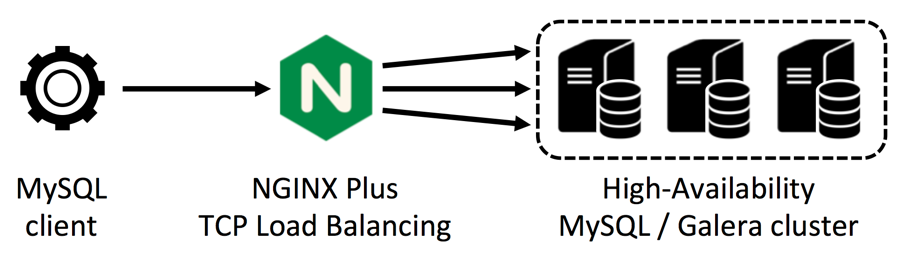
\includegraphics[width=\linewidth]{images/nginx-plus-load-balancing.png}
     \caption{Діаграма компонентів комунікації Nginx та Galera кластеру для MySql баз даних.}
     \label{fig:nginx_mysql}
\end{figure}

То ж, ми можем зробити висновок, що у цій архітектурі налаштування балансувальнику Nginx для комунікації с базами даних можлива. Подібні рішення будут працювати і з Mongo DB, Postgres, Percona та іншими. 

Теперь ми пропонуємо розібратись, чи підтримує Nginx динмічне балансування. 
Nginx PLUS реалізує динамічне балансування за допомогою груп серверів (upstream servers) таким чином: конфігурація серверів у групі може змінбватися динамічно за допомогою Nginx Plus REST API інтерфейсу. Адміністратор мережі може дивится сервери у групах або передивится конфігурацію конкретного серверу, змінювати параметри серверу, а також додавати або видаляти сервери за допомогою HTTP запитів на NGINX Plus REST API.
Остання опція - це і є той ключ, який задовільняю потреби алгоритму. 

Тобто, наразі NGINX Plus підходить за всіма параметрами, але якщо знадобиться поширювати функціонал реалізації нашого основного механізму, це неможливо буде зробити на стороні NGINX Plus, бо NGINX Plus - комерційне забезпечення, хоча і є продуктом NGINX reverse proxy - веб-серверу з можливостями статичного балансування з відкритим джерелом коду. Хоча є можливість реалізувати інший модифікований протокол балансування для узгодженості в NGINX proxy, але це потребує й реалізації алгоритму динамічного балансування, бо NGINX proxy підтримує тільки статичні алгоритми. Для цього приведемо порівняльну характеристику Nginx - Nginx Plus
(http://linuxbsdos.com/2015/09/25/nginx-plus-vs-open-source-nginx/ ) (див.\ref{fig:nginx_nginx_plus} )

\begin{figure}
\centering
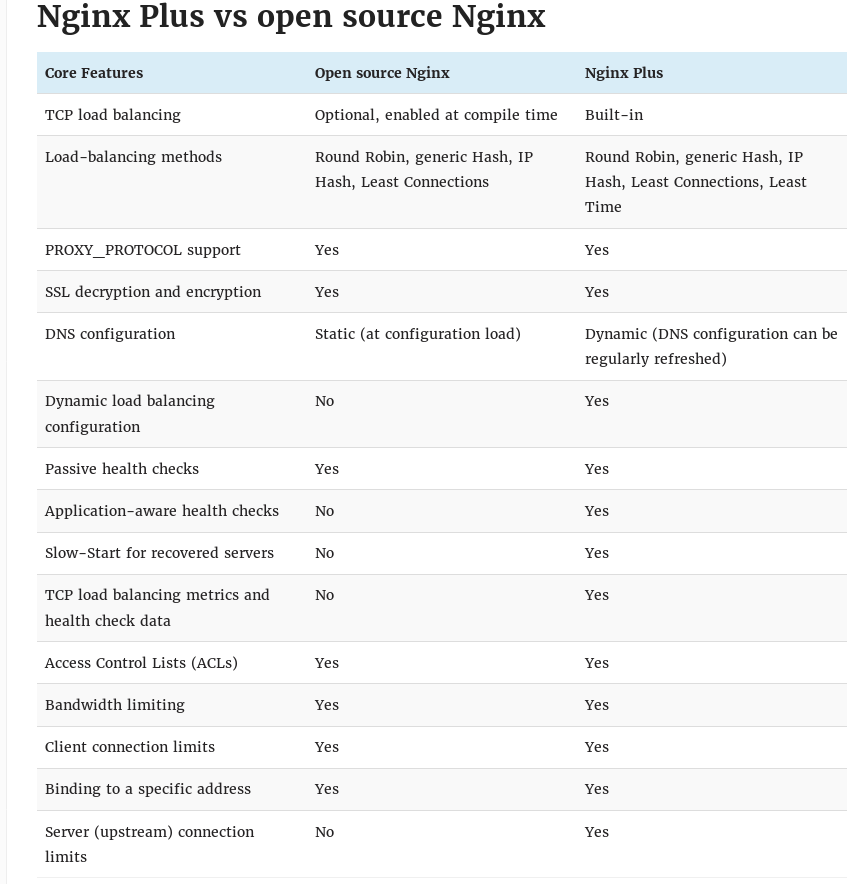
\includegraphics[width=\linewidth]{images/compare_nginx_nginx_plus.png}
     \caption{Порівняльна характеристика можливостей балансування навантаження у Nginx та NGINX Plus.}
     \label{fig:nginx_nginx_plus}
\end{figure}

\subsection{HAProxy}

HAProxy - програмне забезпечення з відкритим джерелом коду, проксі-сервер з високим рівнем доступності, який підтримує балансування в системі HTTP/TCP серверів, в тому числі і динамічне.
HAProxy забезпечує комунцікацію з базами даних за схожим принципом, що і NGINX Plus. Наступна діаграма компонентів описує один із прикладів архітектури, яку можуть побудувати адміністратори мережі розподіленої бази даних (див. Малюнок \ref{fig:haproxy_mysql}):

\begin{figure}
\centering
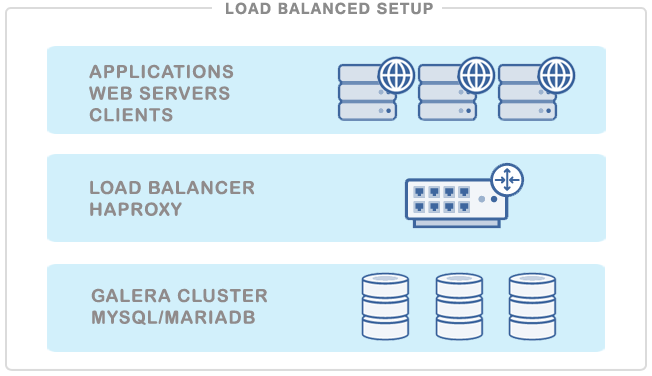
\includegraphics[width=\linewidth]{images/haproxy_database_balancing.png}
     \caption{Діаграма компонентів комунікації HAProxy з вузлами бази даних MySQL}
     \label{fig:haproxy_mysql}
\end{figure}


Оскільки HAProxy - найбільш потужна реалізація балансувальника навантаження, ми можем роздивитись діаграму компонентів більш детально для огляду можливостей, які можуть стати нам у нагоді.

Клієнтська програма, яка спирається на базу даних на "бекенді" (вузел, який відповідає за серверну частину виконання запиту), може легко переповнити базу даних багатьма запланованими паралельними з'єднаннями. HAProxy забезпечує чергу та регулявання підключень до одного або декількох серверів MySQL і запобігає перевантаженню одного сервера надто великою кількістю запитів. Всі клієнти підключаються до примірника HAProxy, а зворотний проксі-сервер (reverse proxy) пересилає з'єднання з одним з доступних серверів MySQL на основі алгоритму балансування завантаження.

За допомогою HAProxy в класі балансування навантаження ми матимемо наступні переваги:

\begin{itemize}
\item Усі програми мають доступ до кластера за допомогою однієї IP-адреси або імені хосту. Топологія кластеру баз даних маскується за HAProxy.
\item З'єднання MySQL є збалансованими між завантаженими вузлами БД.
\item Можна додавати або видаляти вузли бази даних без будь-яких змін у програмах. 
\item Після досягнення максимальної кількості з'єднань в базах даних (в MySQL), HAProxy чергує додаткові нові підключення. Це добре зроблений спосіб регулювання запитів на з'єднання з базою даних і забезпечує захист від перевантажень.

\end{itemize}

ClusterControl підтримує розгортання HAProxy одразу з інтерфейсу користувача, і за замовчуванням він підтримує три алгоритми балансування навантаження - roundrobin, least connection або source. Користувачам рекомендується мати HAProxy між клієнтами та пулом серверів баз даних, особливо для кластерів Galera або MySQL Cluster, де запити на "бекенди" обробляються однаково.

Також можна налаштувати перевірку HAProxy, яка перевіряє, чи підключений сервер, просто підключившись до порту MySQL (як правило, 3306).

Найкращий спосіб перевірки здоров'я MySQL - це використання власного сценарію ("скрипт" у цьому випадку), який визначає наявність сервера MySQL, ретельно вивчаючи його внутрішній стан, який залежить від використовуваного рішення кластеризації. За замовчуванням ClusterControl надає власну версію сценарію перевірки здоров'я, яка називається mysqlchk, яка розташована на кожному сервері MySQL у наборі балансування навантаження, і має можливість повернути статус HTTP-відповіді та (або) стандартний вихід (stdout), який корисний для перевірки стану здоров'я на рівні TCP.
Нижче ми описуємо приклад власної реалізації перевірки стану здоров'я для серверів баз даних у розподіленому сховищі та демонструємо факт, що налаштування потрібної поведінки можлива.
\begin{example} mysqlchk для Galera Cluster. Якщо сервери сервера MySQL пройшли перевірку стану, то скрипт поверне простий HTTP 200 код статусу OK зі статусом виходу 0. А інакше скрипт поверне 503 Сервіс недоступний і статус завершення 1.
Використання $xinetd$ - це найпростіший спосіб отримати сценарій перевірки стану здоров'я, зробивши його демоном та прослуховуючи спеціальний порт (за замовчуванням - 9200). Після цього HAProxy підключиться до цього порту і запитає про вихід перевірки здоров'я. Якщо метод перевірки стану - httpchk, HAProxy буде шукати код відповіді HTTP, і якщо метод tcp-check, він буде шукати очікуваний рядок.

Наведена нижче блок-схема ілюструє процес звітування про стан здоров'я вузла Galera для встановлення декількох майстрів (див. \ref{fig:mysqlchk}).

\begin{figure}
\centering
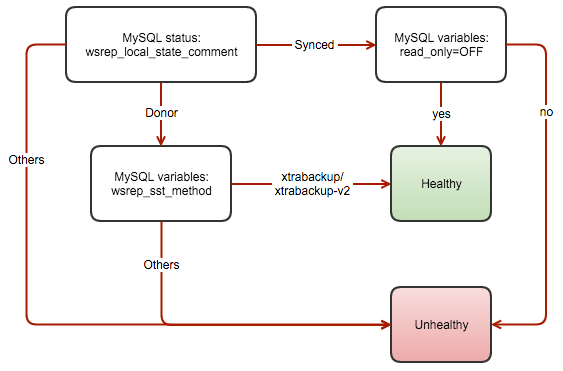
\includegraphics[width=\linewidth]{images/mysqlchk.png}
     \caption{Діаграма активності перевірки працездатності (healthcheck) вузлу бази даних з наявністю налаштованого HAProxy серверу}
     \label{fig:mysqlchk}
\end{figure}
\end{example}
https://severalnines.com/resources/tutorials/mysql-load-balancing-haproxy-tutorial

Відповідно до того, що сказано вище (стаття [18]) , є можливість для адміністратора мережі написати власну реалізацію перевірки працездатності для бази даних, тобто таблиця здорових (в нашому випадку, здорових і узгоджених) вузлів буде змінюватися за цим алгоритмом. 

Варто зауважити, що перевірка працездатності виконується HAProxy з конфігурованою періодичністю, 
тобто адміністратор розподіленої мережі бази даних також може цим керувати.


HAProxy, як і NGINX Plus , підтримує конфігурацію кластерів серверів, тобто відповідні одиниці даних сервери можуть бути об'єднані у кластери. 
Для цього потрібно сконфігурувати необхідну кількість бекендів, де кожний бекенд (backend) може відповідати за кластер. 

Також HAProxy реалізує механізм, відомий як комутація на основі контенту, який реалізується за 
допомогою контрольного списку доступу (ACL - Access Control List).
Спершу зробимо визначення ACL:

Більшість операцій у HAProxy можуть бути виконаними з певними умовами. Ці умови будуються через комбінації кількох контрольних списків доступу, використовуючи логічні оператори (AND, OR, NOT). Кожний такий список є серією тестів, які основані на таких елементах:

\begin{itemize}

\item спосіб вилучення методу для вилучення елемента для тестування; ;

\item необов'язкова серія перетворювачів для перетворення елемента ;

\item список відповідних шаблонів ;

\item відповідний метод, який вказує, як порівнювати шаблони із зразком

\end{itemize}

Тепер вертаєючись до механізму комутації контенту, можемо описати і його: принцип цього механізму полягає у наступному: 
коли відбувається з'єднання (connection) або запит (request) , запит або з'єднання містить в собі деяка інформацію, яка може впливати на те, який бекенд (група вузлів) буде вибраний для цього запиту. Це реалізується за допомогою умов на основі ACL. Тобто якщо інформація, яку містить запит чи з'єднання, відповідає умовам ACL, то може бути вибраний певний бекенд.


Отже, ми можемо побачити, що HAProxy має надзвичайно гнучку конфігурацію, що дозволяє нам сформувати відповідну модель роботи з балансуванням навантаження між узгодженими вузлами для певної одиниці даних.

\subsection{Інші балансувальники}

Ми роздивилися найбільш популярні, потужні, багатофункціональні балансувальники навантаження  з гнучкою конфігурацією. Але є інші балансувальники, які теж варті уваги. Ми оглянемо їх у цьому підрозділі і вирішимо, чи існує можливість використовувати їх для меїанізму балансування між узгодженими вузлами.
\begin{itemize}

\item Seesaw. Це балансувальник навантаження, розроблений компанією Google. Проблема полягає в тому, що цей балансувальник задовільняє лише потреби Google. Але так чи інакше він не має такого гнучкого функціоналу для того, щоб конфігурувати систему балансування за нашими вимогами. [30]
https://opensource.googleblog.com/2016/01/seesaw-scalable-and-robust-load.html

\item Traefik. Traefik - це сучасний HTTP зворотній проксі-сервер для мікросервісів. Traefik легко інтугрується з існуючим стеком компонентів інфраструктури в системі (Docker, Swarm mode, Kubernetes, Marathon, Consul, Etcd, Rancher, Amazon ECS, ...) і налаштовується автоматично і динамічно. Опція 
and configures itself automatically and dynamically. Pointing Traefik на компоненти оркестрації - це єдиний необхідний крок налаштування. Але Traefik не підтримує балансування для баз даних, та не може бути задіяний у використанні з іншими компонентами, які будуть служити посередниками між Traefik та вузлами бази даних.
https://docs.traefik.io/

\item Neutrino. Neutrino - розробка eBay PaaS команди. Neutrino повторює у багатьох елементів функціональності HAProxy, бо перед тим, як розробляти цей балансувальник команда eBay стояли перед вибором: віддати перевагу рішенню HAProxy чи розробити власний балансувальник.  [31]
https://www.ebayinc.com/stories/blogs/tech/announcing-neutrino-for-load-balancing-and-l7-switching/ . Рішення розробити Neutrino було вибрано за таких причин:
HAProxy не задовільнив вимогам для комутації між вузлами на рівні HTTP, базуючись на деяких специфічних правилах, 
відправки журналу повідомлень на кінцеві точки (endpoints) API (Application programming interface) , а також можливість додавання нових алгоритмів балансування.

Завдяки тому, що Neutrino, як і HAProxy, підтримує балансування і на рівні HTTP, і на рівні TCP, може бути використане рішення кластеру Galera, 
та приклад диаграми компонентів може мати такий самий вигляд, як і для HAProxy та NGINX Plus (див. Малюнки \ref{fig:haproxy_mysql} та \ref{fig:nginx_mysql}).
Окрім того, Neutrino - також рішення з відкритим джерелом коду, єдиний недолік - це те, що Neutrino підтримує менш функціоналу, ніж HAProxy та NGINX Plus, і механізм балансування між узгодженими вузлами, використаний разом з цим балансувальником, може мати більшу складність. 

\end{itemize}

Отже, з балансувальників, які ми роздивилися, ми можемо вибрати три, реалізувати математичні та імітаційні моделі, в яких одним з компонентом буде той чи інший балансувальник. 


Також у наступних розділах робиться оцінка кожної моделі. Також доведемо, що моделі, які містять тільки компоненти з програмного забезпечення балансувальників та повністю реалізують потрібний нам механізм, не існують.

Між тим ми розглянемо варіант моделі розподіленої бази даних, яка зовсім не має в якості компоненту жодного програмного забезпечення балансування навантаження, визначимо переваги та недоліки такої моделі і також зробимо її оцінку.

В кінці кінців це допоможе нам зробити оптимальне рішення та вибрати модель, яка найбільш відповідає нашим вимогам і має найменший показник складності алгоритму, який може бути реалізований за цією моделлю.

\section{Хеш-таблиці для зберігання узгоджених вузлів}

Перед тим, як приступити к моделюванню розподіленої баз даних з участю механізму балансування між ухгодженими вузлами, також необхідно зробити визначення рішення хеш-таблиць та роль яка відводиться їм у рішеннях з балансуванням. 

Отже, {\bfseries Хеш-таблиця } або {\bfseries хеш-відображення } - структура даних, що реалізує інтерфейс асоціативного масиву, а саме, вона дозволяє зберігати пари (ключ, значення) і здійснювати три операції: операцію додавання нової пари, операцію пошуку і операцію видалення за ключем. Існує два основних варіанта хеш-таблиць: з ланцюжками і з відкритою адресацією. Хеш-таблиця містить в собі деякий масив H, елементами якого є пари (хеш-таблиця з відкритою адресацією) або списки пар (хеш-таблиця з ланцюжками).

Виконання операцій в хеш-таблиці починається з обчислення хеш-функції від ключа. Отримане хеш-значення i = hash(key) відіграє роль індексу в масиві H. Після цього операція (додавання, видалення, пошук) перенаправляється об'єктові, який зберігається у відповідній комірці масиву H[i].

Ситуація, коли для різних ключів отримується одне й те саме хеш-значення, називається колізією. Такі події непоодинокі — наприклад, при додаванні в хеш-таблицю розміром 365 комірок усього лише 23-х елементів ймовірність колізії вже перевищує 50 відсотків (якщо кожний елемент може з однаковою ймовірністю потрапити в будь-яку комірку)  — див. парадокс днів народження. Через це механізм розв'язання колізій — важлива складова будь-якої хеш-таблиці.

В деяких особливих випадках вдається взагалі уникнути колізій. Наприклад, якщо всі ключі елементів відомі заздалегідь (або дуже рідко змінюються), тоді для них можна знайти деяку досконалу хеш-функцію, яка розподілить їх за комірками хеш-таблиці без колізій. Хеш-таблиці, які використовують подібні хеш-функції, не потребують механізму розв'язання колізій, і називаються хеш-таблицями з прямою адресацією. 

Роздивимося хеш-таблицю більш детально: 

\paragraph{\textbf{Постановка задачі}}
[36] 
%http://elcat.pnpu.edu.ua/docs/%D0%90%D0%BB%D0%B3%D0%BE%D1%80%D0%B8%D1%82%D0%BC%D0%B8%20%D1%96%20%D1%81%D1%82%D1%80%D1%83%D0%BA%D1%82%D1%83%D1%80%D0%B8%20%D0%B4%D0%B0%D0%BD%D0%B8%D1%85/lab12-13_table.html
У хеш-таблиці замість безпосереднього використання ключа як індексу масиву, індекс обчислюється за значенням ключа. 
Функція, що відображає елемент множини ключів ${0, 1, ..., n-1}$ на множину індексів ${0, 1, ..., m-1}$, $(m <n)$, 
називається хеш-функцією. 
Якщо два ключі хешуються в одну й ту саму комірку, то говорять про виникнення колізії. За способом вирішення колізій розрізняють:
\begin{itemize}
\item відкрите хешування — усі елементи, що хешуються в одну комірку, об’єднуються у зв’язний список. При відкритому хешуванні хеш-таблиця є масивом, кожна комірка якого містить покажчики на заголовок списку всіх елементів, хеш-значення ключа яких дорівнює індексу комірки. 
\item закрите хешування — усі елементи зберігаються безпосередньо у хеш-таблиці, при потраплянні у зайняту комірку обирається послідовність інших хеш-значень. 
При закритому хешуванні хеш-таблиця є масивом, елементи якого занумеровані від 0 до m-1.
\end{itemize}


Необхідно забезпечити для хеш-таблиці реалізацію основних операторів:
\begin{itemize}
\item пошук елемента;
\item запис елемента;
\item читання елемента. 
\end{itemize}

\paragraph{Існуючі рішення для хеш-таблиць}

\section{Моделі власного механізму та його оцінка}
В цьому розділі ми зробимо концептуальні моделі та моделі компонентів для рішення маршрутизації між узгодженими нодами без задіяння відомого програмного забезпечення балансувальників навантаження, щоб мати повну картину для оцінювання у подальших розділах.

Зараз ми представляємо математичну модель для розподіленої бази даних.
Ми визначаємо її як кортеж компонентів $(N, L, \partial,D, r)$, де \\

\begin{tabular*}{\textwidth}{cp{0.5cm}p{0.8\textwidth}}\label{tb:mm_first}
$N$&& - кінцева множина вузлів розподіленій бази даних; \\
$L$&& - кінцева множина посилань (зв'язків) між вузлами у розподіленiй базі даних; \\
$\partial:L\rightarrow 2^N$&& - відображення, яке  сполучає кожне посилання з двома вузлами у мережі розподіленої бази даних;\\
$D$&& - кінцева множина зберігаємих нероздільних одиниць даних залежачи від побудованої схеми розподіленої бази даних та принципу розподілення у тий чи іншій конфігурації;\\
$r:D\rightarrow 2^N$&& - відображення, яке ассоціює кожну одиницю даних $d$ з підмножиною вузлів, які зберігають репліку такої одиниці даних; \\

$R(d)$&& - кінцева множина реплік (версій) $r$ даної одиниці даних $d$;\\
$N(d)$&& - кінцева множина вузлів, які зберігають репліку даної одиниці даних $d$; \\
$l(N(d))$&& - кількість вузлів у розподіленій базі даних, які зберігають репліку даної одиниці даних $d$; \\
$n_c$&& - кількість вузлів підмножини $N_d$, де всі вузли зберігають одну і ту ж версію одиниці даних.

$D:$
\end{tabular*}

У цьому розділі ми розширимо існуючу модель визначенням:

\begin{definition}
$N(c, d)$ - кінцева множина вузлів підмножини $N(d)$, де всі вузли зберігають одну і ту ж версію одиниці даних, тобто одну і ту ж репліку. Це визначає множину вузлів, які узгоджені між собою відповідно до одиниці даних $d$.


\end{definition}

Цю модель найбільш точно відображує наступна діаграма компонентів (див. Малюнок \ref{fig:d_components_without_lb}).


\begin{figure}
\centering

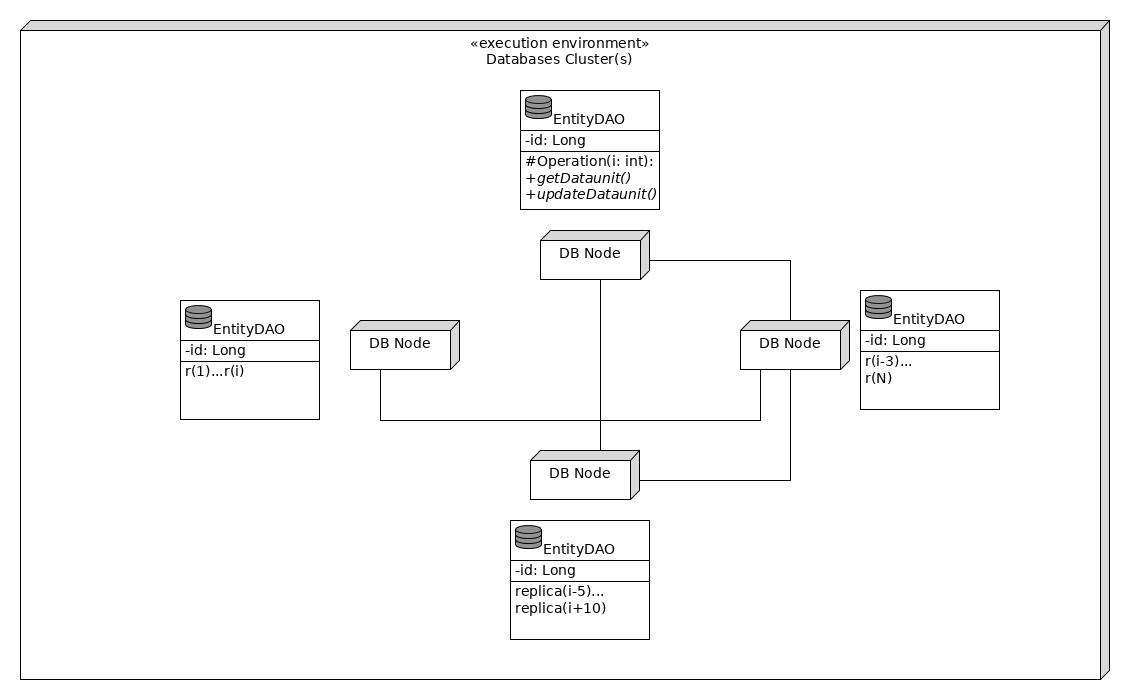
\includegraphics[width=\linewidth]{images/d_component_without_lb.jpg}
     \caption{Діаграма компонентів розподіленого сховища без балансувальника навантаження.}
     \label{fig:d_components_without_lb}
\end{figure}

Також ми представляємо концептуальну модель і діаграму послідовності, за допомогою яких буде будуватися імітаційна модель для цього зразку математичної моделі (див. Малюнок \ref{fig:d_concepts_without_lb} і Малюнок \ref{fig:d_sequence_without_lb})
\begin{figure}
\centering

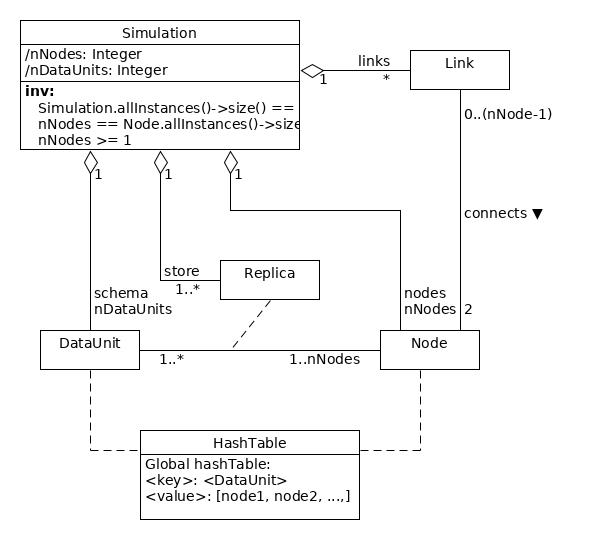
\includegraphics[width=\linewidth]{images/d_concept_without_lb.jpg}
     \caption{Діаграма концептів розподіленого сховища без балансувальника навантаження.}
     \label{fig:d_concepts_without_lb}
\end{figure}


\begin{figure}
\centering

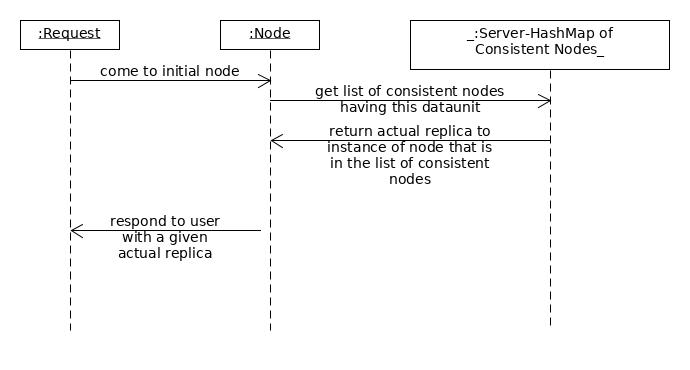
\includegraphics[width=\linewidth]{images/d_sequence_without_lb.jpg}
     \caption{Діаграма послідовності розподіленого сховища без балансувальника навантаження.}
     \label{fig:d_sequence_without_lb}
\end{figure}

Після побудування моделей, крім імітаційної, ми можемо зробити висновки про переваги та недоліки такого алгоритму:

\begin{itemize}
\item Переваги
\begin{itemize}
\item Незалежність від іншого програмного забезпечення, оскільки це рішення не використовує жодних сторонніх  глобальних рішень
\item Простота реалізації. Таке рішення не є ресурсо-витратним, щоб реалізувати такий алгоритм, потрібен сервер (кластер) с хеш-таблицею, яка буде містити список вузлів за конкретною одиницею даних (побудова такої таблиці може залежити від того, як одиниці даних розподілені між вузлами мережі розподіленого сховища)

\end{itemize}
\begin{itemize}
\item Ненадійність. Такий механізм не є надійним, бо неможливо гарантувати працездатність всіх узгоджених вузлів у хеш-таблиці, і так чи інакше цей алгоритм потребує періодичну перевірку стану вузлів, тому що з того часу, як вузел став узгодженим, він міг вийти із зони доступності. Зону доступності (availability) може гарантувати періодична перевірка стану вузлів. Однак такий механізм може використовуватися, якщо адміністратор мережі і бізнес-аналітики проекту, компонентом якого  розподілена база за цією моделлю, можуть гарантувати таку доступність вузлів та зв'язків між ними (або знайти рішення, яке буде це гарантувати), що після запиту на запис вузел не вийде з зони доступності, або запити на запис відбуваються з таким коротким інтервалом, що це до дозволить в цей же час перевіряти і стан вузлів одночасно с оновленням хеш-таблиці.
\item Залежність кожного вузла один від одного. Вузли повинні спілкуватися між собою за епідеміологічними алгоритмами
\end{itemize}
\end{itemize}

Щоб довести це, ми побудували імітаційну модель (див. Додатки) за побудованими раніше концептуальной діаграмою та діаграмою послідовності.

У якості глобальної Хеш-таблиці ми вибрали Redis (порівняльна характеристика різних рішень хеш-таблиць представлена у другому розділі поточної глави).

\section{Моделі гібрідного механізму з використанням балансувальника}
Побудувавши математичну, концептуальну та імітаційну модель у минулому розділі, ми будемо дотримуватися такої самої стратегії для гібрідного рішення.
Оскільки кожний балансувальник різний, що ми вже показали у першому розділі цієї глави, ми повинні врахувати цей факт при побудуванні моделей для цього рішення та, можливо, зробити кілька варіантів моделей для кожного з вибраних балансувальників. 

Першою моделлю, яку ми опишемо, стане модель для балансування між узгодженими вузлами, базуючись на програмному рішенні HAProxy.

Отже, модель розподіленої системи даних у цьому рішенні поширюється іншими компонентами, які необхідні для перевірки стану вузлів та балансування між ними.
Посилаючись на вже розроблену модель для розподіленої бази даних (див. Модель у минулому розділі \ref{tb:mm_first}), ми додаємо такі елементи:

\begin{tabular*}{\textwidth}{cp{0.5cm}p{0.8\textwidth}}\label{tb:mm_second}
$SLB frontend$&& - потужний сервер або група потужних серверів, які відповідають за балансування и мають встановлений сервер балансувальника HAProxy, відповідаючи за обробку запитів. Запит на запис повинен виконуватися таким самим чином, як би він виконувався у будь-якій розподіленій системі бази даних. У випадку запита на читання, балансувальник повинен опрацювати запит налаштованих умов контрольного списку доступу та направити запит на відповідний $SLB backend$;\\
$SLB backend$&& - кінцева множина кластерів для розподіленої бази даних, які повинні опрацювати запит.

\end{tabular*}

Тепер роздивимося спрощений варіант діаграми компонентів для цієї моделі (див. Малюнок \ref{fig:d_components_lb}). Варто зауважити, що для чистоти зображення на цій діаграмі не вказані зв'язки між вузлами, бо це відноситься до того принципу, як розповсюджуються репліки між вузлами мережі розподіленої бази даних, а не до механізму роботи кластера балансувальника та кластерів вузлів РБД. Однак цей факт буде відображений у наступній діаграмі. (див Малюнок \ref{fig:d_concept_lb}). 

\begin{figure}
\centering

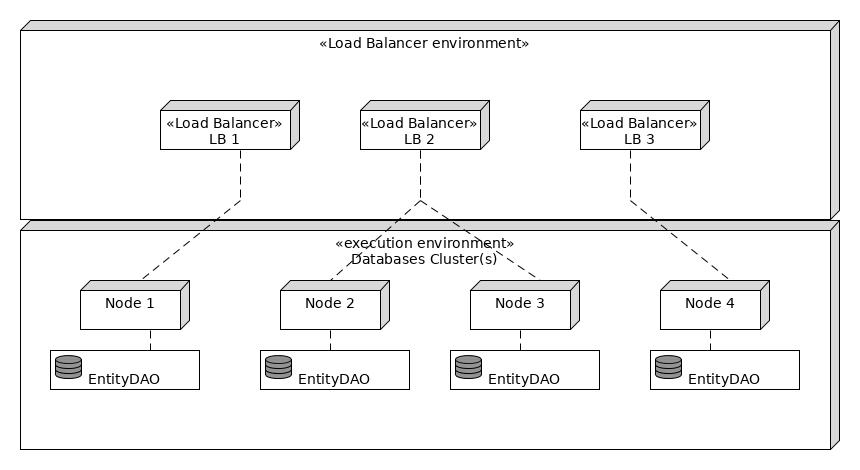
\includegraphics[width=\linewidth]{images/d_components_lb.jpg}
     \caption{Діаграма 	компонентів розподіленого сховища за участі балансувальника навантаження.}
     \label{fig:d_components_lb}
\end{figure}

\begin{figure}
\centering

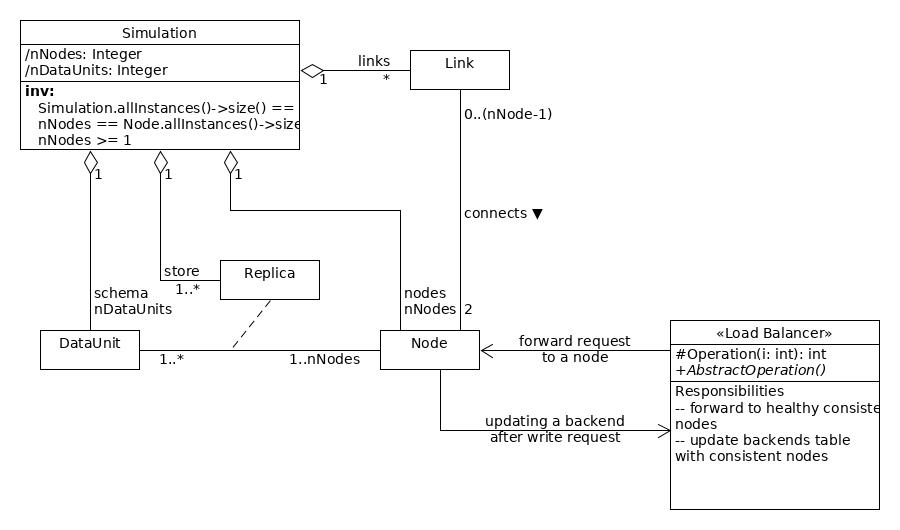
\includegraphics[width=\linewidth]{images/d_concept_lb.jpg}
     \caption{Діаграма 	концептів розподіленого сховища за участі балансувальника навантаження.}
     \label{fig:d_concept_lb}
\end{figure}


Наступні діаграми, яку хотілося б презентувати, є діаграми послідовності для розподіленого сховища даних за участі рішення балансувальника.
Ці діаграми розділені на кілька частин, де перша діаграма презентує програмне рішення для розподіленого сховища (див. Малюнок \ref{fig:d_sequence_lb}), а друга - інфраструктурне рішення, яке показує більш детально рекомендації для налаштування балансувальника навантаження

\begin{figure}
\centering

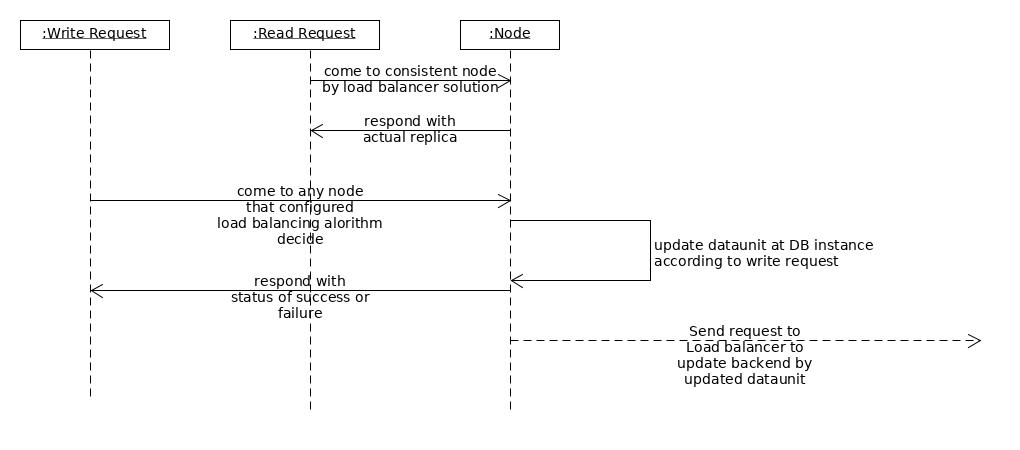
\includegraphics[width=\linewidth]{images/d_sequence_lb.jpg}
     \caption{Діаграма 	послідовності розподіленого сховища за участі балансувальника навантаження. Програмне рішення}
     \label{fig:d_sequence_lb}
\end{figure}

Наступні діаграми можуть мати декілька варіантів реалізації, оскільки ми описуємо можливості використання декількох реалізацій балансувальника навантаження,
і кожне з них може бути налаштовано зовсім різними методами, існуючими у той чи іншій реалізації. 

Для кожного рішення балансувальника буде два варіанти реалізації механізму: використання існуючих алгоритмів балансування та використання опцій налаштування самого балансувальника, щоб задовільнити потреби механізму або написання нового алгоритму балансування.

\noindent То ж спочатку ми опишемо рішення балансування з використанням HAProxy (див. Діаграму \ref{fig:d_sequence_lb_configuration}). 

\begin{figure}
\centering

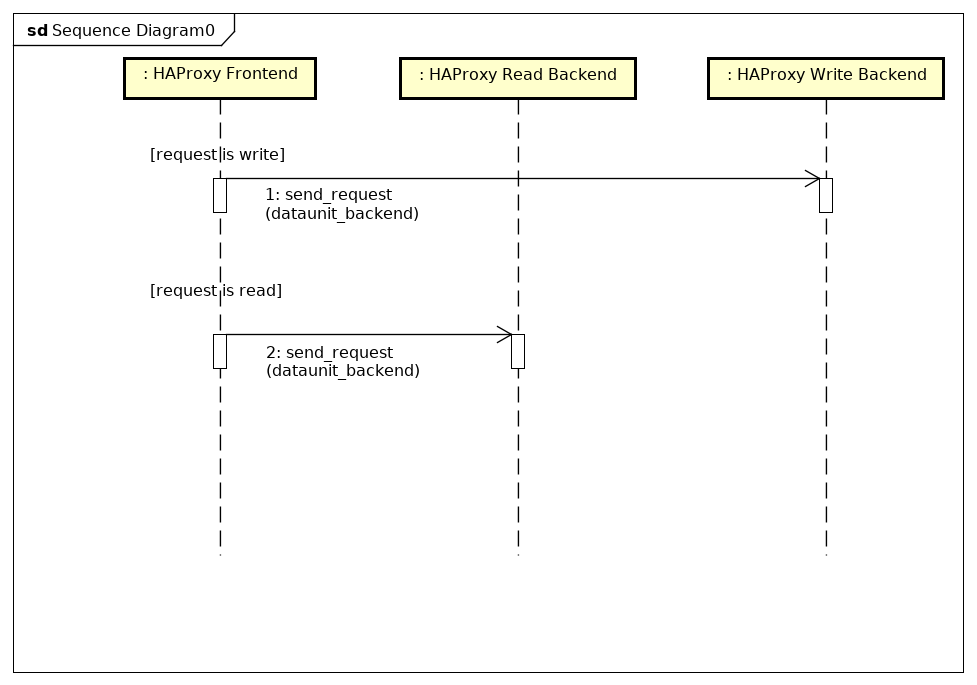
\includegraphics[width=\linewidth]{images/Sequence_Diagram_haproxy.png}
     \caption{Діаграма 	послідовності механізму налаштування HAProxy для балансування навантаження у розподіленому сховищі}
     \label{fig:d_sequence_lb_configuration}
\end{figure}

Діаграма не повністю демонструє даний механізм, то ж ми опишемо кілька деталей:

\begin{enumerate}

\item Клієнт посилає запит до бази даних, вказуючи цільову одиницю даних
\item Коли запит приходить на балансувальник, HAProxy відповідно до наданої конфігурації очікує або запит на читання, або запит на запис. Оскільки ми працюємо  с tcp запитом, необхідно використовувати більш низькорівневі операції, щоб зрозуміти, на який бекенд перенаправити запит за відповідною одиницею даних $d$. TCP запит має параметр $payload$, за допомогою якого можна дізнатися , яка одиниця даних прийшла на запит. Таким чином запит буде пересланий на бекенд (
або ж групу серверів) за відповідною одиницею даних. Для цього файл налаштування $/etc/haproxy/haproxy.cfg$ буде містити такі рядки: 

\begin{lstlisting}[language=bash,caption={bash version}]

backend dataunit_1
  mode tcp
  option tcp-check
  balance roundrobin
  server server1 <ip>:<port>
  server server2 <ip>:<port>
  ....
  server server_n <ip>:<port>

backend dataunit_2
  mode tcp
  option tcp-check
  balance roundrobin
  server server1 <ip>:<port>
  server server2 <ip>:<port>
  server server3 <ip>:<port>
  .....
  server server_n <ip>:<port>
 
....

backend dataunit_n
  server server1 <ip>:<port>
  server server2 <ip>:<port>
  server server3 <ip>:<port>
  .....
  server server_n <ip>:<port>
 

\end{lstlisting}

\item Тепер пояснимо, як вузли у різних $backend$ можуть динмаічно змінюватися, видалятися та додаватися нові. Таку можливіст забезпечує HAProxy Runtime API (див. https://www.haproxy.com/blog/dynamic-configuration-haproxy-runtime-api/). Отже, щойно екземпляр бази даних модифікував репліку, запит про те що, операція на запис пройшла успішно, відправиться на сервер поруч с сервером HAPRoxy (в одному кластері, або навіть на одному сервері), додаток, який слухає такі запити, за допомогою HAProxy Runtime API оновить $backend$ за відповідною одиницею даних, якщо дана репліка з відповідним часовим показником вважається найновішою. Таким чином конфігурація HAProxy буде динамічно змінюватися із зростанням кількості повністю узгоджених вузлів. Складності можуть виникнути, якщо запити за цією одиницею даних 
відбуваються частіше, ніж HAProxy config встигає збільшувати кількість узгоджених вузлів у відповідному $backend$. Це має показати оцінка такого алгоритму.
 
\item Для зберігання версій реплік за часовим показником буде використовуватися хеш-таблиця, де ключом є одиницею даних, а значення за цим ключом представляю собою одиницю даних $t1$, порівняну з одиницею даних, яка використовується у системі для відстеження часу. Кількість ключів у такій хеш-таблиці також залежить від обсягу пам'яті, які дозволено використовувати для даної хеш-таблиці. Це означає, що кількість одиниць даних обмежується обсягом пам'яті, виділеної для хеш-таблиці.

\end{enumerate}

Ще одне рішення про використання балансувальника навантаження для балансування між узгодженими вузлами - це власний незалежний алгоритм балансування для будь-якого з балансувальників. Перевагами такого рішення є незалежність від існуючих алгоритмів балансування, чітке і стабільне виконання поставленої задачі, можливість побудувати модульну архітектуру, не залежачи від можливостей налаштувань балансувальника, використання системи балансування за призначенням.
Недоліком є складність реалізації.

Наступна діаграма демонструє такий алгоритм у поєднанні з механізмом оновлення списку узгоджених вузлів за відповідною одиницею даних. (див. Малюнок \ref{fig:d_sequence_lb_custom_algorithm}) .

\begin{figure}
\centering

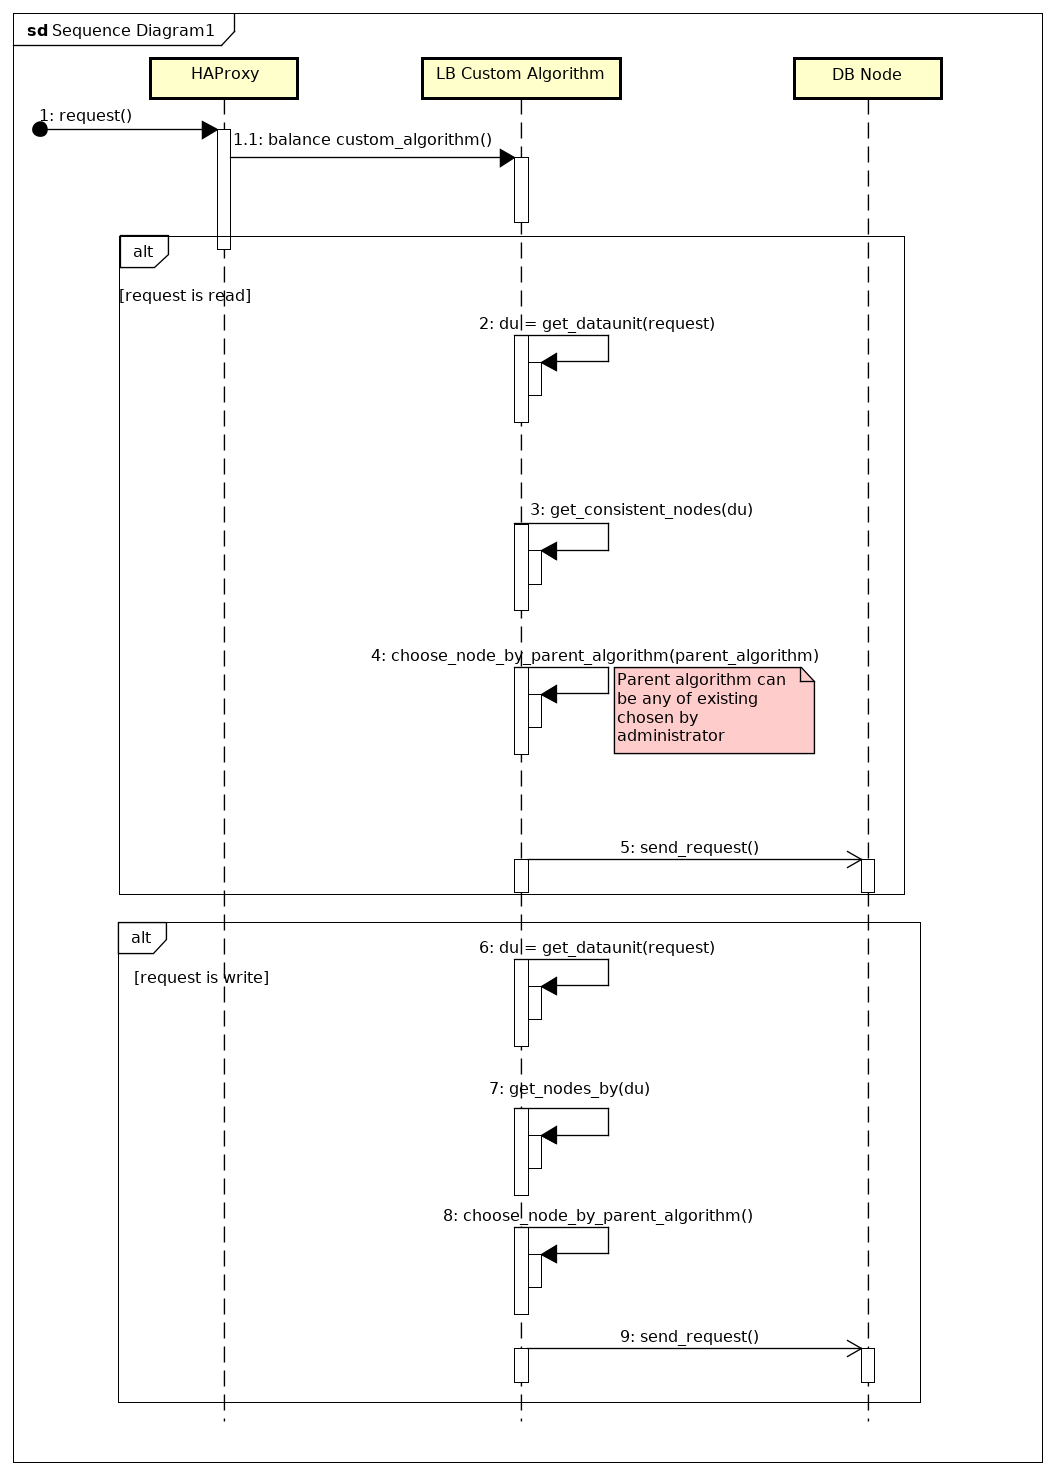
\includegraphics[width=\linewidth]{images/sequence_diagram_lb_custom_algorithm.png}
     \caption{Діаграма 	послідовності власного алгоритму балансування у будь-якому балансувальнику для балансування навантаження у розподіленому сховищі}
     \label{fig:d_sequence_lb_custom_algorithm}
\end{figure}


\section{Оцінка несуперечливості та доступності за застосованими моделями} \label{efficiency_estimates}
https://www.arangodb.com/2018/02/nosql-performance-benchmark-2018-mongodb-postgresql-orientdb-neo4j-arangodb/

В минулих секціях ми розробили три варіанти механізмів для рішення питання несуперечливості у розподілених базах даних, не втрачаючи доступності.
У цій секції ми запустили імітаційні моделі за розробленими механізмами і побудували графіки, які дозволяють оцінити кожен з алгоритмів відповідно рохробленому механізму.
При оцінюванні алгоритмів участь взяли еталонні тести використаних рішень , таких як, Redis, HAProxy, обчислений середній час серед еталонних тестів у різних системах керування базами даних (час обробки запитів на запис та читання.
При оцінюванні також ми пропонуємо ввести так званий поріг доступності (availability threshold) - мінімальну кількість вузлів, узгоджених між собою відповідно заданої одиниці даних. Ця опція може конфігуруватися адміністратором розподіленої бази даних. 

У нашій симуляції на першій групі графіків (див. Малюнки \ref{fig:lb_custom_10}, \ref{fig:lb_custom_100}, \ref{fig:lb_custom_3000},\ref{fig:lb_custom_5000}) такий поріг дорівнює 30 вузлам на одиницю даних
і відображений на графіках прямою лінією. Перший графік відображає власний балансувальний алгоритм для існуючого балансувальника, який модифікує список вузлів за одиницею даних та використовує за цими вузлами вказаний існуючий алгоритм (least connection, round robin тощо). 

Друга група графіків (див. Малюнки \ref{fig:lb_haproxy_config_10}, \ref{fig:lb_haproxy_config_100}, \ref{fig:lb_haproxy_config_3000},\ref{fig:lb_haproxy_configuration_5000}) відображує механізм налаштування HAProxy , HAProxy Rest API та кластеру будь-якої СКБД. Принцип полягає у тому, що балансувальник знає, за яку одиницю даних відповідає кожна з динамічних груп серверів. Кожний сервер бази даних, окрім СКБД, має налаштований сервер, який обробляє запити таким чином, що після оновлення репліки має можливість надіслати запис на HAProxy Rest API запит на модифікування відповідної групи серверів, а також протягом неперервного процесу поширення реплік надсилає також запити на HAProxy Rest API на додавання поточного серверу у групу узгоджених між собою вузлів. При цьому на серверів HAProxy і HAProxy Rest API відбувається перевірка, чи є дана репліка результатом першого оновлення або репліка прийшла в процесі поширення реплік на інші вузли.

І, нарешті, третя група графіків відображує оцінку третього алгоритму, де балансування відбувається тільки за допомогою центрального серверу, який утримує хег-таблицю для узгоджених вузлів та хеш-таблицю реплік, а також приймає запити на оновлення від вузлів с СКБД та відправляє  запити на випадковий вузел з наявного списку (див. Малюнки \ref{fig:own_alg_10}, \ref{fig:own_alg_100}, \ref{fig:own_alg_3000},\ref{fig:own_alg_5000}).

\begin{figure}
\centering

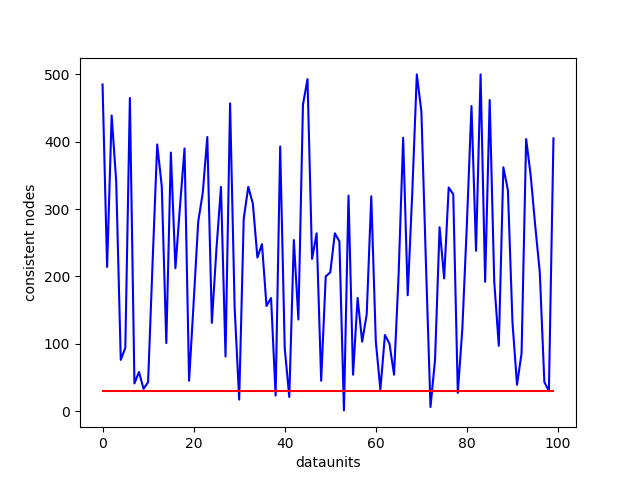
\includegraphics[width=\linewidth]{images/lb_custom/w_10_r_500.png}

     \caption{Оцінка власного алгоритму для існуючого балансувальника}
     \label{fig:lb_custom_10}
\end{figure}


\begin{figure}
\centering

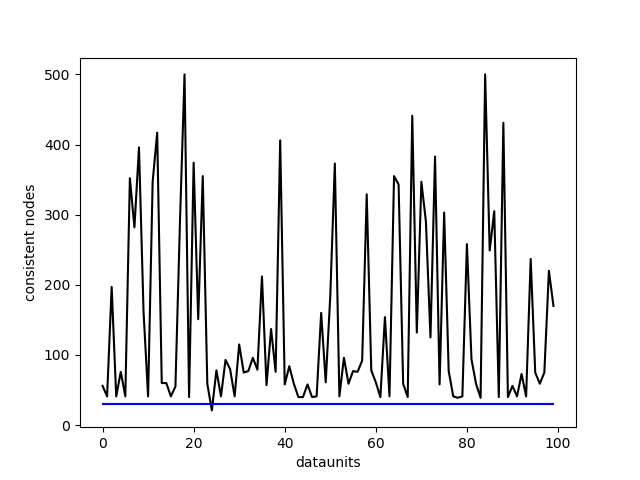
\includegraphics[width=\linewidth]{images/lb_custom/w_100_r_500.png}

     \caption{Оцінка власного алгоритму для існуючого балансувальника}
     \label{fig:lb_custom_100}
\end{figure}

\begin{figure}
\centering

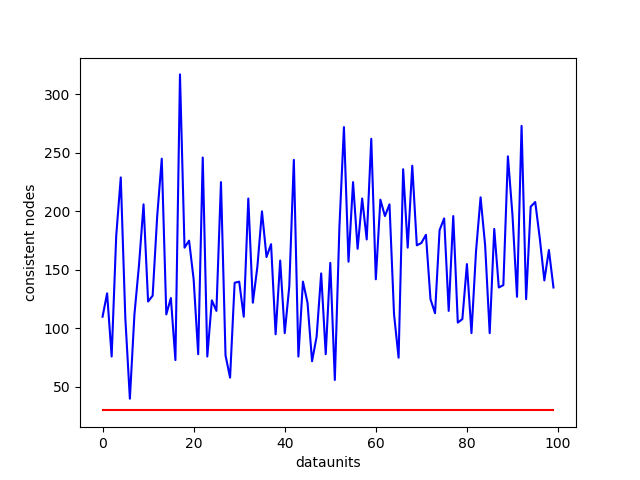
\includegraphics[width=\linewidth]{images/lb_custom/w_3000_r_500.png}

     \caption{Оцінка власного алгоритму для існуючого балансувальника}
     \label{fig:lb_custom_3000}
\end{figure}

\begin{figure}
\centering

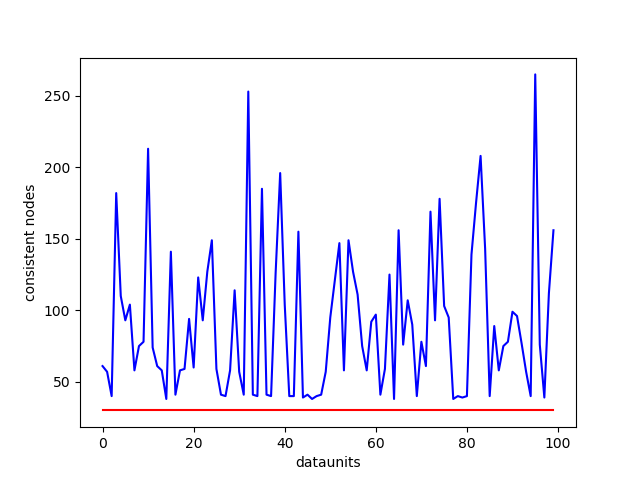
\includegraphics[width=\linewidth]{images/lb_custom/w_5000_r_500.png}

     \caption{Оцінка власного алгоритму для існуючого балансувальника}
     \label{fig:lb_custom_5000}
\end{figure}

%%%%%%%%%%%%%%%%%%%%%%%%%%%%% Друга група графіків


\begin{figure}
\centering

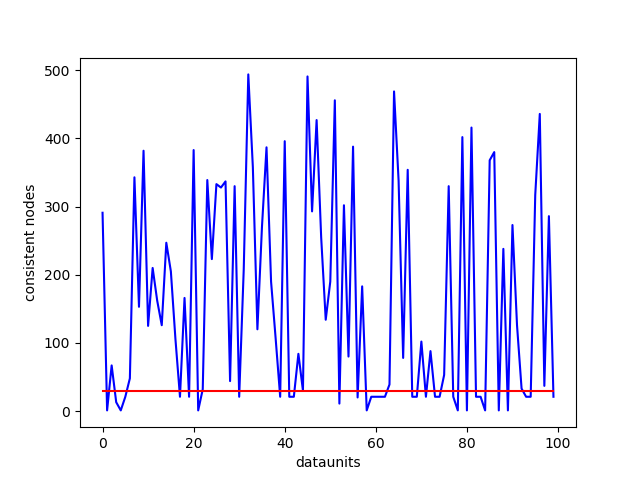
\includegraphics[width=\linewidth]{images/lb_haproxy_configuration/w_10_r_500.png}

     \caption{Оцінка алгоритму з використанням можливостей налаштування для існуючого балансувальника}
     \label{fig:lb_haproxy_config_10}
\end{figure}

\begin{figure}
\centering

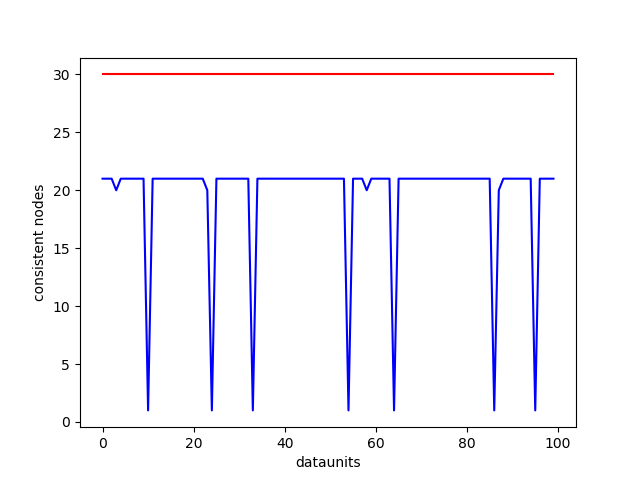
\includegraphics[width=\linewidth]{images/lb_haproxy_configuration/w_100_r_500.png}

     \caption{Оцінка алгоритму з використанням можливостей налаштування для існуючого балансувальника}
     \label{fig:lb_haproxy_config_100}
\end{figure}

\begin{figure}
\centering

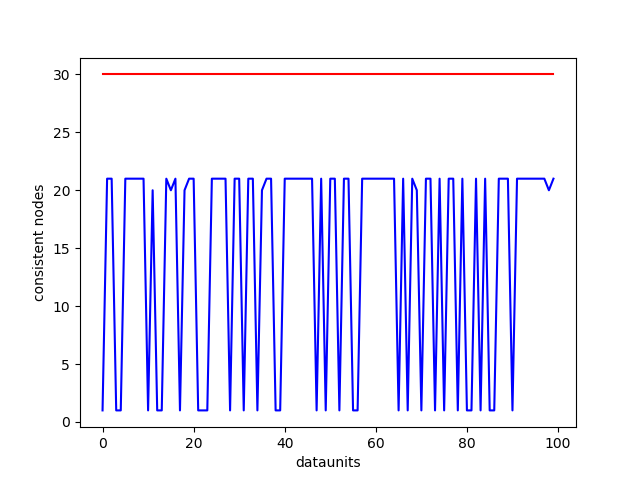
\includegraphics[width=\linewidth]{images/lb_haproxy_configuration/w_3000_r_500.png}

     \caption{Оцінка алгоритму з використанням можливостей налаштування для існуючого балансувальника}
     \label{fig:lb_haproxy_config_3000}
\end{figure}

\begin{figure}
\centering

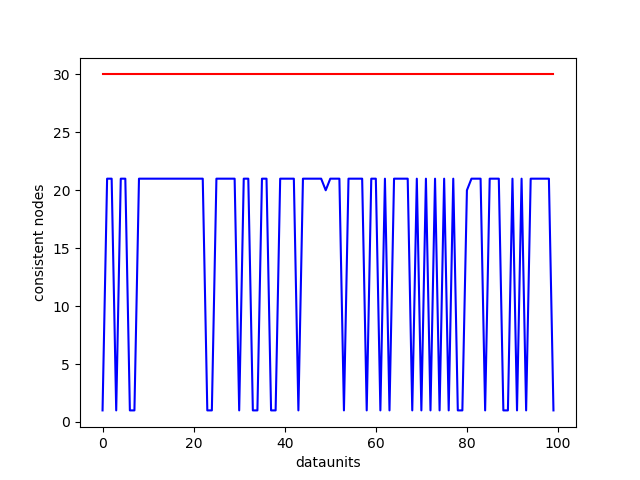
\includegraphics[width=\linewidth]{images/lb_haproxy_configuration/w_5000_r_500.png}

     \caption{Оцінка алгоритму з використанням можливостей налаштування для існуючого балансувальника}
     \label{fig:lb_haproxy_config_5000}
\end{figure}

%%%%%%%%%%%%%%%%%%%%%%%%%%%% Третя група графіків

\begin{figure}
\centering

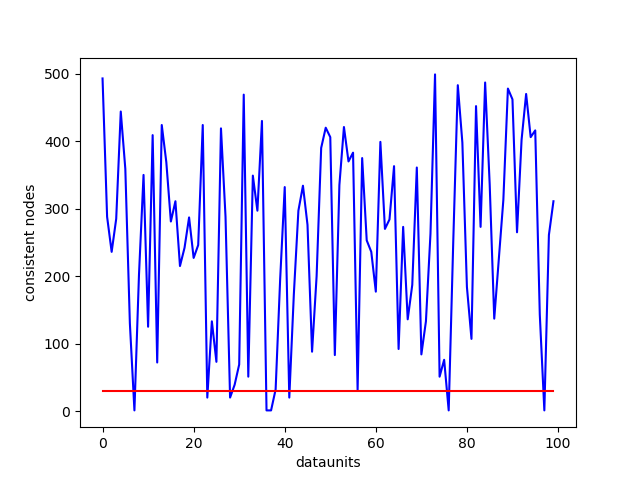
\includegraphics[width=\linewidth]{images/own_balancing/w_10_r_500.png}

     \caption{Оцінка алгоритму з використанням можливостей налаштування для існуючого балансувальника}
     \label{fig:own_alg_10}
\end{figure}

\begin{figure}
\centering

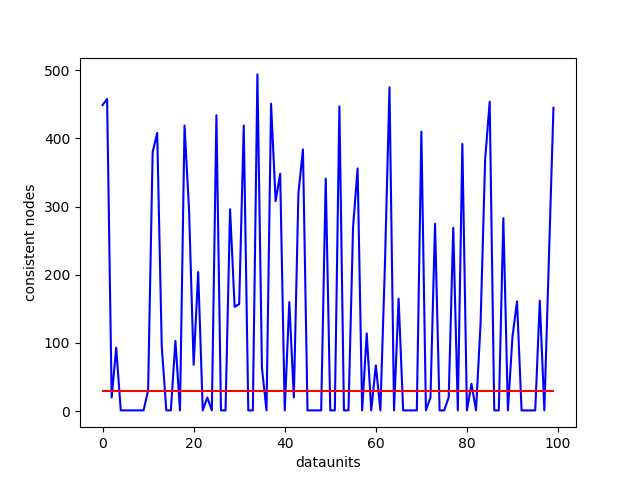
\includegraphics[width=\linewidth]{images/own_balancing/w_100_r_500.png}

     \caption{Оцінка алгоритму з використанням можливостей налаштування для існуючого балансувальника}
     \label{fig:own_alg_100}
\end{figure}

\begin{figure}
\centering

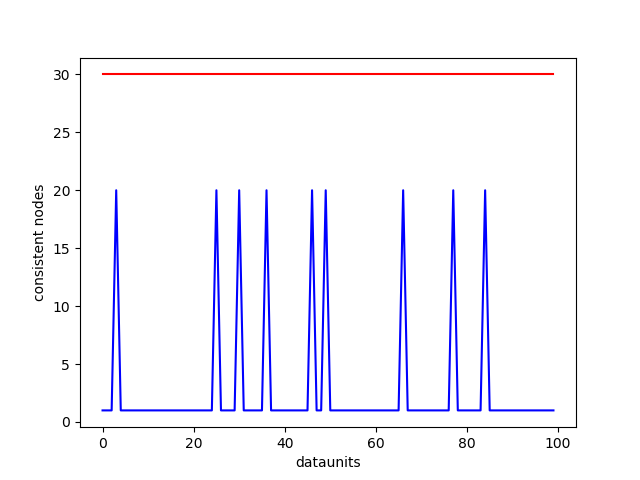
\includegraphics[width=\linewidth]{images/own_balancing/w_3000_r_500.png}

     \caption{Оцінка алгоритму з використанням можливостей налаштування для існуючого балансувальника}
     \label{fig:own_alg_3000}
\end{figure}

\begin{figure}
\centering

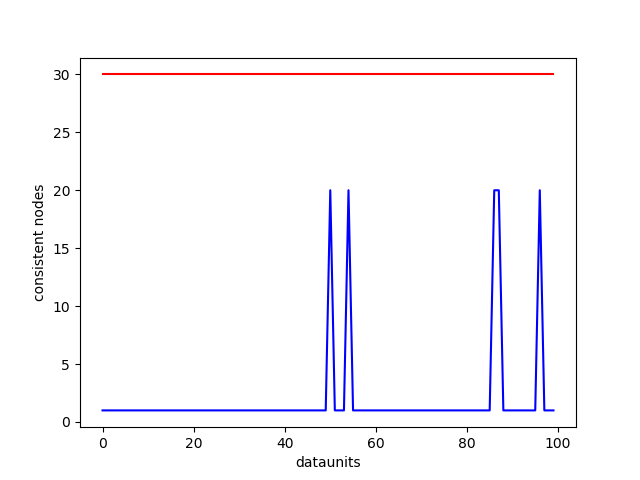
\includegraphics[width=\linewidth]{images/own_balancing/w_5000_r_500.png}

     \caption{Оцінка алгоритму з використанням можливостей налаштування для існуючого балансувальника}
     \label{fig:own_alg_5000}
\end{figure}

Теперь про еталонні показники 
\chapter{Дослідження часу збіжності несуперечливості у ідеальному сховищі}

\chapter{Висновки}
Тож підведемо підсумок виконаної роботи.

Давно з'ясовано, що існує протиріччя підходів ACID / BASE.
Підтримуючи ACID та завжди прив'язуючись до централізованого сховища, можна гарантувати повну узгодженість для бази даних.
Але у такому випадку сервер (кластер) є вузьким місцем (bottleneck) у системі.
Переходячи на BASE и разносячи базу даних на кілька серверів, маємо протилежний підхід, де узгодженість є згодом через якийсь період часу,
тобто повна узгодженість може гарантуватися через певний період часу. З цим ми отримуємо більш можливість горизонтального масштабування та
підвищення значення доступності бази даних.


Оскільки завдяки CAP-теоремі ми знаємо, що неможливо задовільнити всі три характеристики для бази даних, що, підвищуючи значення однієї характеристики,
втрачаємо значення
для іншої, у цій роботі ми дослідили механізм для обчислення кожної з трьох метрік з CAP-теореми
(узгодженості, доступності та толерантності до розподілень), побудували математичну модель та дали математичне визначення.

Побудовані концептуальні моделі для розподіленої бази даних та імітаційна модель, яка є базисом для всіх експериментів, проведених
у роботі.


Поставлена гіпотеза про зв'язок збіжності узгодженості у розподіленому сховищі та діаметру графа, який відображає топологію сховища.
За допомогою імітаційної моделі побудовані відповідні графіки.


Тож підведемо підсумок виконаної роботи.

Давно з'ясовано, що існує протиріччя підходів ACID / BASE.
Підтримуючи ACID та завжди прив'язуючись до централізованого сховища, можна гарантувати повну узгодженість для бази даних.
Але у такому випадку сервер (кластер) є вузьким місцем (bottleneck) у системі.
Переходячи на BASE и разносячи базу даних на кілька серверів, маємо протилежний підхід, де узгодженість є згодом через якийсь період часу,
тобто повна узгодженість може гарантуватися через певний період часу. З цим ми отримуємо більш можливість горизонтального масштабування та
підвищення значення доступності бази даних.


Оскільки завдяки CAP-теоремі ми знаємо, що неможливо задовільнити всі три характеристики для бази даних, що, підвищуючи значення однієї характеристики,
втрачаємо значення
для іншої, у цій роботі ми дослідили механізм для обчислення кожної з трьох метрік з CAP-теореми
(узгодженості, доступності та толерантності до розподілень), побудували математичну модель та дали математичне визначення.

Побудовані концептуальні моделі для розподіленої бази даних та імітаційна модель, яка є базисом для всіх експериментів, проведених
у роботі.


Поставлена гіпотеза про зв'язок збіжності узгодженості у розподіленому сховищі та діаметру графа, який відображає топологію сховища.
За допомогою імітаційної моделі побудовані відповідні графіки.


Написаний концепт для нового алгоритму, який дозволяє підтримувати майже повну узгодженість, при тому значення доступності для бази
не переходить нижче бажаного порогу. Алгоритм дозволяє балансувати між цими критеріями, не втрачаючи багато на жодному з них.

Алгоритм написаний у трьох варіаціях, по кожної з них проведено дослідження, наскільки можлива реалізація концепту, побудовані концептуальні
та імітаційні моделі для кожної з варіацій алгоритму.

Ідея алгоритму виходить з ідеї балансування між узгодженими вузлами, ідея полягає в тому, щоб по можливості віддавати тільки інформацію з
вузлів які вже отримали нову інформацію и система йде к тому, що нова інформація вже розповсюджується.
Також ідея полягає у тому, що швидкість розповсюдження інформації більше у будь-якому випадку, ніж періодичність запитів до бази даних.
Розповсюдження повідомлень про оновлення - це такі ж самі запити, які надсилає і користувач до бази. То ж у найгіршому випадку
(інтервал між запитами на запис на зміну одиниці даних < швидкість розповсюдження повідомлення до сусідів) матимемо вузьке місце, бо найновішим
буде тільки один вузол. У такому випадку просто будуть відповідати інші вільні вузли. Тобто у найгіршому випадку зберігається узгодженість згодом.
У кращому і середньому випадках ми зможемо підвищити значення узгодженості таким чином, що будуть відповідати не будь-які вузли, а на рівні системи
є можливість вирішити, які вузли відповідатимуть на  запит певної одиниці даних.

Для алгоритму досліджені готові рішення балансування і підтримка такого механізму або можливість його подальшого розвитку, а також розширення алгоритму
і використання його. Побудовані відповідні імітаційні моделі та обчислення ефективності алгоритмів.

 \section{Виконані задачі}
 
 Для досягнення цієї мети у роботі поставлені наступні задачі:

\begin{enumerate}[widest=9999,itemindent=*,leftmargin=0pt]
\item Винесена гіпотеза  про зв'язок диаметру графу з топологією мережі бази даних та часу збіжності бази даних до узгодженого стану
\item Дослідження властивостей розподілених систем, зокрема, розподілених сховищ
\item Дослідження критеріїв розподілених баз даних: узгодженості, доступності, стійкості
\item Аналіз типів узгодженості
\item Аналіз алгоритмів розповсюдження реплік
\item Побудова математичної моделі для розподіленого сховщиа даних, складені  метріки для оцінювання CAP-характеристик
\item Сформовані методи оцінки метрик для оцінювання CAP-характеристик
\item Доказ гіпотези про швидкість розповсюдження реплік для "ідеальної" моделі розподіленої бази даних  
\item Модель балансування узгоджених реплік для підвищення значення метріки критерію узгодженості так, щоб  

\end{enumerate}

І як підсумок, внесли наступні вкладення:

\begin{enumerate}[widest=9999,itemindent=*,leftmargin=0pt]

\item Імітаційна модель для механізму забезпечення узгодженого стану для розподіленої системи
\item Використання алгоритмів балансування  Использование алгоритмов балансировки нагрузки для нового направления
\item Побудова нового алгоритму, який дозволяє значно підвищити значення узгодженості в бази даних, не втрачаючи доступності (
якщо вважати за доступність бази певний поріг для кількості доступних вузлів) до розподіленої бази даних і досягнути бажаного компромісу.
Алгоритм може застосовуватися на етапі формування, проектування бази даних і її налаштування.
\item Оцінки ефективності алгоритму представлені у розділі \ref{efficiency_estimates} у вигляді графіків, отримані за допомою побудованої раніше імітаційної моделі.

\end{enumerate}
 \section{Потенціал використання моделей балансування узгодженості в розподілених сховищах даних}
 \section{Майбутні задачі}

\begin{thebibliography}{99}
% ---A---
\bibitem{bib:database_principles}
 — 
C.J. Date: 
An Introduction to Database Systems. 8th edition.
%
\bibitem{bib:database_integrity}
Г.Ладиженський:
Распределенные информационные системы и базы данных.
Конференция
http://citforum.ru/database/kbd96/45.shtml

\bibitem{bib:tanenbaum_distributed}
Aho, A. V., Sethi, R., Ullman, J. D.: 
Compilers: Principles, Techniques, and Tools (1st ed.). 
Addison-Wesley. ISBN 9780201100884 
(1986).
%
\bibitem{bib:algorithms_epidemic}



\end{thebibliography}
\end{document}
